\chapter{Reasoning RL}
\label{ch:reasoning-rl}
\raggedbottom

In September 2024, OpenAI described a new model family trained to ``think'' before answering: o1 spent more test-time computation on hard problems and substantially improved performance on math, programming, and science benchmarks~\cite{openai2024reasoning}. Four months later, DeepSeek described two closely related systems. \textbf{R1-Zero} was the striking ablation: starting from a base model, it used large-scale reinforcement learning from verifiable rewards without a supervised fine-tuning cold start for reasoning traces. \textbf{R1} was the production-quality recipe: it added cold-start data, multi-stage training, and distillation on top of the RL signal~\cite{deepseekai2025r1}. During R1-Zero training, the model developed behaviors that looked familiar to human problem solvers: longer chains of thought, self-checking, backtracking, and revising a plan after detecting an error.

The striking part was not that RL had been applied to language models. Chapters~\ref{ch:rl-foundations} and~\ref{ch:rlhf} already taught that. The striking part was the \emph{reward source}. In RLHF, the model optimizes against a learned proxy for human preference. In reasoning RL, many tasks have a verifier: a math answer is correct or incorrect; a code solution passes unit tests or fails; a proof checker accepts or rejects a formal proof. The reward is still a design choice, and it can still be gamed, but it is no longer a reward model extrapolating from human comparisons. This chapter studies what changes when the reward becomes verifiable.

Think of the progression from Chapter~\ref{ch:rlhf} to this chapter as moving from a driving instructor to a race timing system. In RLHF, the instructor scores your maneuvers: smoothness, caution, confidence, helpfulness. The scorecard is learned and imperfect. In reasoning RL, the track has a finish line and a clock. Either you finish the lap within the rules or you do not. That does not make racing easy. You still need a vehicle, a training loop, a safety boundary, and a way to avoid exploiting loopholes in the timing system. But the feedback is sharper, cheaper, and more scalable.

\paragraph{What this chapter covers.} Three questions organize the chapter. First, what makes verifiable reward different from preference reward (\S\ref{sec:rlvr-shift}--\S\ref{sec:verifiable-reward-sources})? Second, how do we optimize language models against those rewards in practice, especially with critic-free methods such as GRPO (\S\ref{sec:grpo}--\S\ref{sec:process-outcome})? Third, what new behaviors and systems emerge when training-time RL combines with inference-time compute (\S\ref{sec:emergent-reasoning}--\S\ref{sec:reasoning-landscape})?

\paragraph{Chapter thesis.} \emph{Reasoning RL is not defined by a particular optimizer. It is defined by the shift from subjective preference proxies to verifiable outcome signals.} GRPO matters because it is a practical way to use those signals without a value model, but the deeper paradigm shift is reward design: when the answer can be checked cheaply and reliably, the model can learn from many attempts, not just from human-written demonstrations.

\paragraph{Running example.} Your Project~3 model is now a 3B instruction-tuned and preference-aligned assistant. In this chapter, you train it on middle-school algebra and small programming tasks. For math, the verifier extracts the final answer and compares it to the ground truth. For code, the verifier runs unit tests. Each prompt produces a group of sampled responses; the verifier scores each response; the optimizer increases the probability of successful trajectories and decreases the probability of failed ones. The details of that loop are the algorithmic core of the chapter.

\begin{figure}[t]
\centering
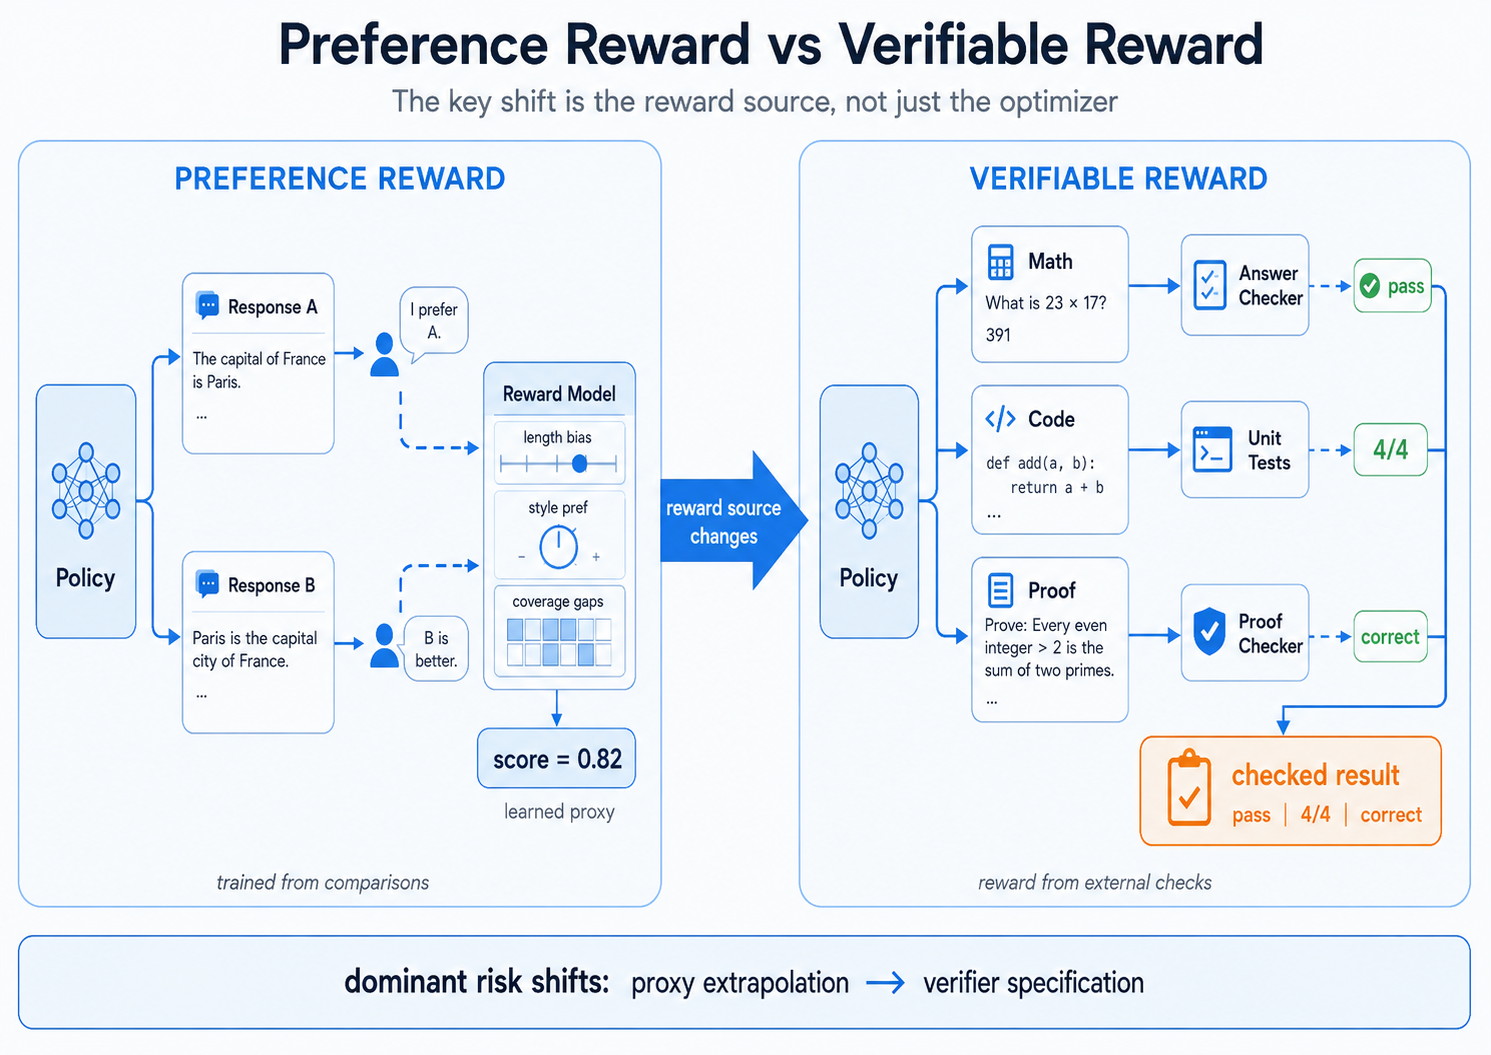
\includegraphics[width=0.95\textwidth]{figures/ch16/fig_rlvr_shift.png}
\caption{\textbf{The shift from preference reward to verifiable reward.} RLHF optimizes against a learned reward model trained on human preferences. Reasoning RL often optimizes against a verifier: exact answer matching, unit tests, formal proof checking, or structured process rewards. The verifier does not eliminate specification risk, but it changes the dominant failure mode from learned-proxy extrapolation to verifier design.}
\label{fig:rlvr-shift}
\end{figure}

\subsection*{Learning Objectives}

After completing this chapter, you should be able to:

\begin{enumerate}
  \item Explain why verifiable rewards change the economics and failure modes of post-training.
  \item Distinguish outcome rewards, process rewards, learned reward models, and self-generated signals.
  \item Derive the GRPO update from the PPO idea by replacing the value model with a group baseline.
  \item Read a reasoning-RL training loop: sampling groups, computing verifier rewards, normalizing advantages, applying token-level policy updates, and monitoring KL.
  \item Explain how RL can induce long reasoning, self-correction, and backtracking without directly imitating human traces.
  \item Connect training-time RL to inference-time scaling methods such as best-of-$N$, majority voting, and search.
\end{enumerate}

\subsection*{Notation}

\begin{center}
\begin{tabular}{ll}
\toprule
Symbol & Meaning \\
\midrule
$x$ & Prompt / problem statement \\
$y_i$ & $i$-th sampled response for the same prompt \\
$G$ & Group size: number of responses sampled per prompt \\
$r_i$ & Verifier reward for response $y_i$ \\
$\bar{r}$, $\sigma_r$ & Mean and standard deviation of rewards within a group \\
$\hat{A}_i$ & Group-relative advantage for response $y_i$ \\
$\rho_{i,t}$ & Token-level probability ratio for response $i$ at token $t$ \\
$\pi_\theta$ & Trainable policy \\
$\pi_{\text{old}}$ & Rollout policy used to sample the current batch \\
$\pi_{\text{ref}}$ & Frozen reference policy used for KL regularization \\
$\beta$ & KL penalty coefficient \\
\bottomrule
\end{tabular}
\end{center}

\subsection*{Timeline of Key Contributions}

\begin{center}
\begin{tabular}{lp{11cm}}
\toprule
Year & Contribution \\
\midrule
2021 & Cobbe et al.\ introduce GSM8K and train verifiers for grade-school math reasoning~\cite{cobbe2021gsm8k}. \\
2022 & STaR bootstraps reasoning by generating rationales, keeping those that lead to correct answers, and fine-tuning iteratively~\cite{zelikman2022star}. \\
2022 & Self-consistency shows that sampling multiple reasoning paths and voting improves chain-of-thought accuracy~\cite{wang2022selfconsistency}. \\
2023 & Lightman et al.\ compare outcome and process supervision and release PRM800K step-level labels~\cite{lightman2023verify}. \\
2023 & ReST frames alignment as an iterative generate-filter-train loop inspired by growing-batch RL~\cite{gulcehre2023rest}. \\
2024 & DeepSeekMath introduces GRPO as a memory-efficient PPO variant for mathematical reasoning~\cite{shao2024deepseekmath}. \\
2024 & OpenAI o1 demonstrates large gains from reinforcement learning that encourages productive chain-of-thought reasoning~\cite{openai2024reasoning}. \\
2025 & DeepSeek-R1 uses GRPO-style RL with verifiable rewards and releases reasoning models and distillations~\cite{deepseekai2025r1}. \\
\bottomrule
\end{tabular}
\end{center}


%----------------------------------------------------------------------
\section{Paradigm Shift: From Preferences to Verifiers}
\label{sec:rlvr-shift}

Chapter~\ref{ch:rlhf} framed RLHF as optimization against an imperfect proxy. The reward model was trained on human comparisons, then frozen. PPO pushed the policy toward responses the reward model scored highly, while KL regularization kept the policy close to the SFT reference. That pipeline works, but it inherits the reward model's blind spots: length bias, sycophancy, overconfidence, and extrapolation outside the distribution where humans labeled comparisons.

Reasoning tasks can change the reward source. For many math, code, and formal tasks, we do not need to ask a human which response they prefer. We can check whether the answer is right. This family of methods is often called \textbf{RL with verifiable rewards} (RLVR): reinforcement learning where the reward comes from a checker, test suite, proof verifier, or other rule-based scoring function rather than a learned preference model.

\subsection{What Becomes Easier}

Verifiable rewards give three practical advantages:

\begin{enumerate}[nosep]
  \item \textbf{Cheap scale.} Once the verifier exists, scoring another response is cheap. A unit test suite can evaluate thousands of code samples without additional human annotation.
  \item \textbf{Lower label noise.} Human preference labels often disagree. Exact-answer math checking has its own extraction problems, but if the answer is parsed correctly, the label is objective.
  \item \textbf{On-policy iteration.} The policy can generate fresh attempts, receive scores immediately, and update on its own distribution. This avoids one major limitation of offline preference data: the training pairs may not match the current policy's behavior.
\end{enumerate}

These advantages explain why reasoning RL can train for many rounds. The model is not waiting for humans to compare every pair. It is attempting problems, seeing which attempts pass, and updating.

\subsection{What Does Not Become Easy}

Verifiable does not mean perfect. A verifier checks what it is designed to check. If the reward extracts only the final answer, it may reward lucky guesses or brittle shortcuts. If code tests are incomplete, a model can overfit hidden assumptions. If a formal proof checker accepts a proof, the result is strong; but formalizing the problem may be the hardest part. The reward is sharper than a preference model, but the specification problem remains.

The race-timing analogy is useful here. A stopwatch is more objective than a driving instructor's opinion, but it does not tell you whether the driver followed every safety rule unless the track instrumentation checks those rules. Objective measurement shifts the problem from label noise to instrumentation design.

\begin{tcolorbox}[colback=blue!5, colframe=blue!40, title=\textbf{Verifiable Reward Moves the Hard Problem, Not Solves It}]
It is tempting to see verifiable reward as alignment without the proxy problem. It is not. It is a shift in where the specification challenge lives. In RLHF, the hard problem is \emph{modeling preferences}: the reward model must approximate human judgment, and it fails when the policy leaves the training distribution. In reasoning RL, the hard problem is \emph{specifying coverage}: the verifier correctly checks what it checks, but it checks nothing else. A model that passes every math test may still be unhelpful, dishonest, or unsafe. A model that passes every unit test may exploit edge cases the tests do not cover.

The strategic question is not ``is the reward real?'' but ``what does this reward not measure?'' RLHF has specification risk in the reward model. Reasoning RL has specification risk in the task boundary. Both need the same engineering discipline: monitor what the optimizer is actually doing, not just the score it achieves.
\end{tcolorbox}

\begin{quickrecap}
\textbf{Quick Recap.}
\begin{itemize}[nosep,leftmargin=1.5em]
  \item RLHF uses learned preference proxies; reasoning RL often uses verifiers.
  \item Verifiers make reward cheaper, less noisy, and easier to apply on-policy.
  \item Verifiable reward changes the failure mode from reward-model extrapolation to verifier specification.
\end{itemize}
\textit{Next: what kinds of verifiers can language models actually use?}
\end{quickrecap}


%----------------------------------------------------------------------
\section{Verifiable Reward Sources}
\label{sec:verifiable-reward-sources}

A verifier is a function that maps a response to a score without asking a human for a new judgment. Some verifiers are exact. Others are only structured proxies. Reasoning RL systems usually combine several reward sources, because a single binary correctness signal is often too sparse.

\begin{figure}[t]
\centering
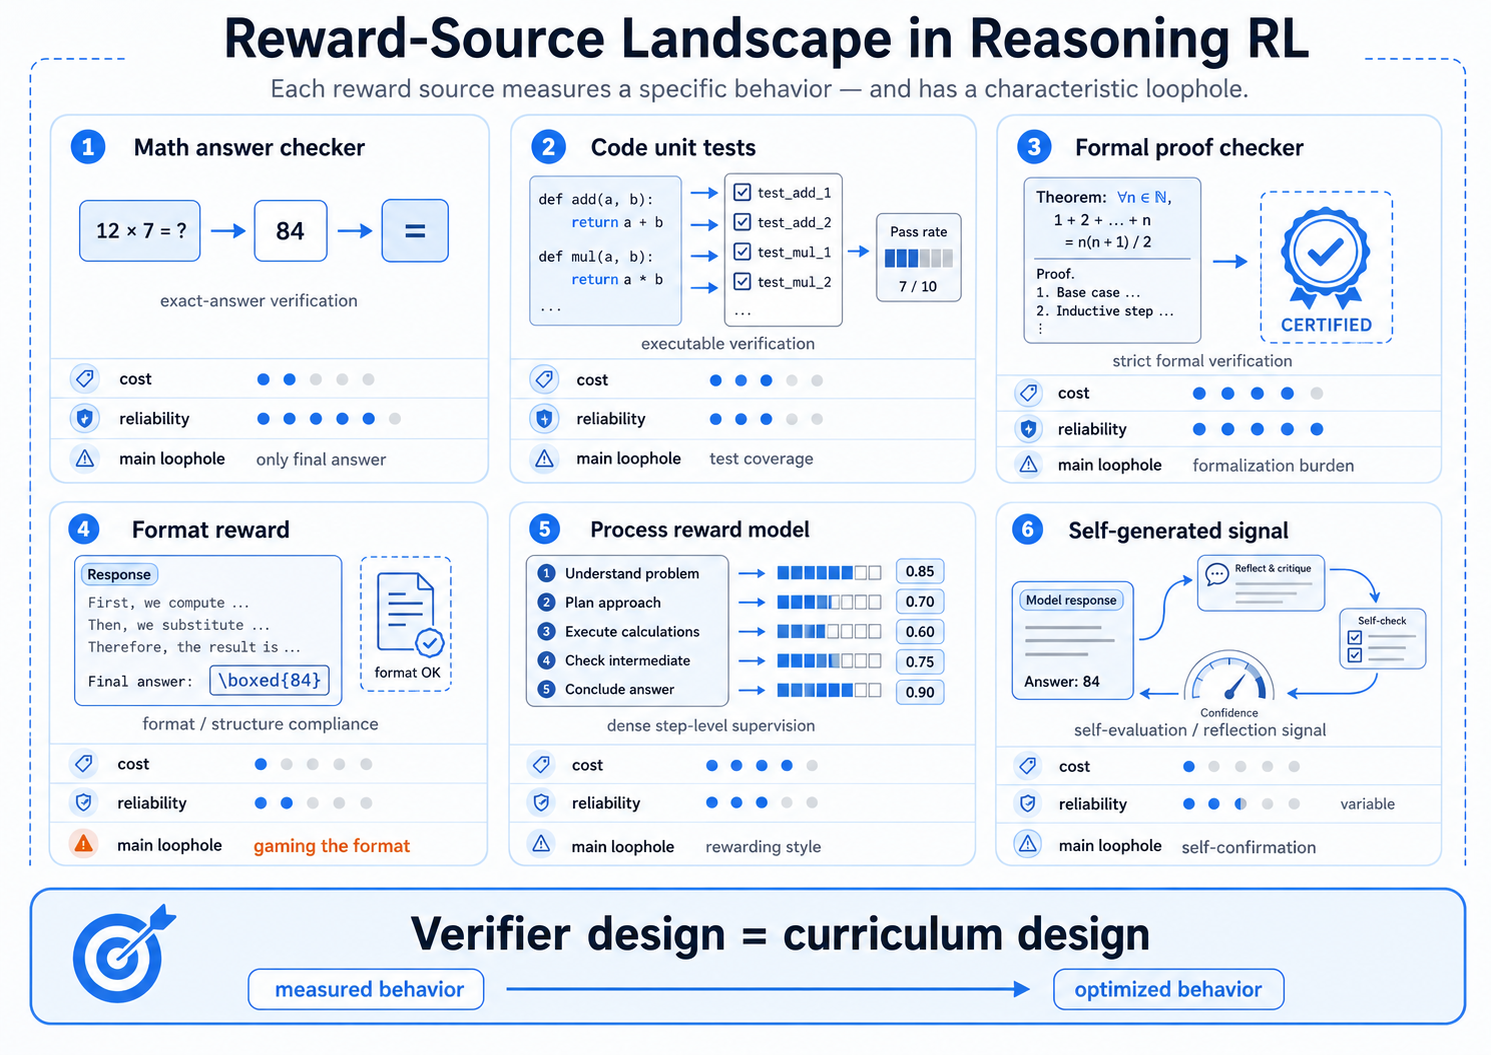
\includegraphics[width=0.95\textwidth]{figures/ch16/fig_verifier_sources.png}
\caption{\textbf{Verifiable reward sources.} Math answer checkers, code unit tests, formal proof checkers, format rewards, process reward models, and self-generated signals differ in cost, reliability, and coverage. The key design question is not ``is the reward objective?'' but ``what behavior does this reward actually measure?''}
\label{fig:verifier-sources}
\end{figure}

\subsection{Outcome Verifiers}

\textbf{Math answer checking} is the canonical example. The model generates a solution and a final answer. The verifier extracts the final answer and compares it to the ground truth. If the answer matches, $r=1$; otherwise $r=0$. The main engineering problems are parsing and equivalence: ``$1/2$'', ``0.5'', and ``$\frac{2}{4}$'' should be treated as the same answer, while a correct-looking expression with a wrong sign should fail.

\textbf{Code unit tests} are another natural verifier. The model writes a program; the verifier runs hidden tests; the reward is the fraction of tests passed or a binary pass/fail. This reward is more informative than exact-answer math because partial credit is possible. But tests are only as good as their coverage. A model can pass weak tests while failing edge cases.

\textbf{Formal verification} is the strongest form: a proof checker accepts or rejects the response. The reward is reliable when the formalization is correct, but the domain coverage is narrow and the setup cost is high.

\subsection{Auxiliary Rewards}

Real systems rarely use only the final correctness bit. They often add auxiliary rewards:

\begin{itemize}[nosep]
  \item \textbf{Format reward}: the response contains a final answer in the required markup, such as \texttt{\textbackslash boxed\{\}}.
  \item \textbf{Length reward or penalty}: the response is neither too short to reason nor so long that it wastes compute.
  \item \textbf{Language quality reward}: the response remains coherent, not just correct.
  \item \textbf{Safety filter}: the response avoids disallowed content even while optimizing a task reward.
  \item \textbf{Diversity reward}: sampled attempts explore different solution paths instead of collapsing to one brittle template.
  \item \textbf{Brevity reward}: code or proof outputs avoid unnecessary length when shorter solutions pass the same verifier.
\end{itemize}

These shaping rewards make the sparse signal denser, but they reintroduce specification risk. If the format reward is too strong, the model learns to produce the format even when the answer is wrong. If the length penalty is too strong, it learns to skip reasoning. The art is to use shaping rewards as guardrails, not as the main objective.

\subsection{The Verifier Contract}

For Project~3, the verifier contract should be explicit:

\begin{itemize}[nosep]
  \item What exactly is parsed from the model response?
  \item What counts as equivalent to the ground-truth answer?
  \item Does the reward give partial credit?
  \item Are invalid formats scored as zero, or as a small negative reward?
  \item Are the training and held-out verifier tests separate?
\end{itemize}

If you cannot answer these questions, you do not have a reward function; you have a hope that the reward matches the task.

\begin{quickrecap}
\textbf{Quick Recap.}
\begin{itemize}[nosep,leftmargin=1.5em]
  \item Math, code, and formal proof tasks provide natural outcome verifiers.
  \item Auxiliary rewards can make training smoother, but they can also become new reward hacks.
  \item The verifier contract should specify parsing, equivalence, partial credit, invalid formats, and train/test separation.
\end{itemize}
\textit{Next: how do we optimize a policy against these verifier rewards without a value model?}
\end{quickrecap}


%----------------------------------------------------------------------
\section[Policy Optimization for Reasoning]{Policy Optimization for Reasoning: PPO, GRPO, and Critic-Free Variants}
\label{sec:grpo}

Chapter~\ref{ch:rl-foundations} introduced PPO, and Chapter~\ref{ch:rlhf} instantiated it for RLHF. PPO uses a value model $V_\psi(s)$ to estimate advantages. That critic is expensive: it is usually a model-sized object, trained alongside the policy, and it must predict the expected return from partial sequences. In reasoning RL with verifiable rewards, a simpler baseline is often available.

The core observation behind GRPO is straightforward: if you sample several responses to the \emph{same prompt}, you can compare them to each other. The group itself provides a baseline. Correct responses are above the group mean; incorrect responses are below it. You can compute advantages without a learned value model.

\subsection{The GRPO Training Step}

For a prompt $x$, sample a group of $G$ responses:

\[
y_1, y_2, \ldots, y_G \sim \pi_{\text{old}}(\cdot \mid x).
\]

Run the verifier on each response and obtain rewards $r_1,\ldots,r_G$. Then compute group-normalized advantages:

\begin{equation}
\label{eq:grpo-advantage}
\hat{A}_i = \frac{r_i - \bar{r}}{\sigma_r + \epsilon_{\text{std}}},
\qquad
\bar{r} = \frac{1}{G}\sum_{j=1}^{G} r_j.
\end{equation}

Here $\epsilon_{\text{std}}$ is a small numerical stabilizer, such as $10^{-8}$, that prevents division by zero when every response in the group receives the same reward. It is not the PPO clipping parameter. That all-equal case is also a training diagnostic: if most groups have $\sigma_r \approx 0$, the task distribution is too easy, too hard, or the sampling temperature is too low.

The policy update is PPO-like and token-level:

\begin{equation}
\label{eq:grpo-loss}
\mathcal{L}_{\text{GRPO}} =
\mathbb{E}\!\left[
\frac{1}{G}\sum_{i=1}^{G}\frac{1}{|y_i|}\sum_{t=1}^{|y_i|}
\min\!\left(
\rho_{i,t}\hat{A}_i,\;
\text{clip}(\rho_{i,t},1-\epsilon_{\text{clip}},1+\epsilon_{\text{clip}})\hat{A}_i
\right)
- \beta D_{\text{KL}}(\pi_\theta \| \pi_{\text{ref}})
\right],
\end{equation}

where

\[
\rho_{i,t} =
\frac{\pi_\theta(y_{i,t}\mid x,y_{i,<t})}
{\pi_{\text{old}}(y_{i,t}\mid x,y_{i,<t})}.
\]

This is the operational detail that matters. The group reward is sequence-level, but the policy update is token-level. Every token in a successful response receives a positive advantage; every token in a below-average response receives a negative advantage. The model is not told which step was responsible. It receives trajectory-level credit and must discover which token patterns correlate with success.

\begin{figure}[t]
\centering
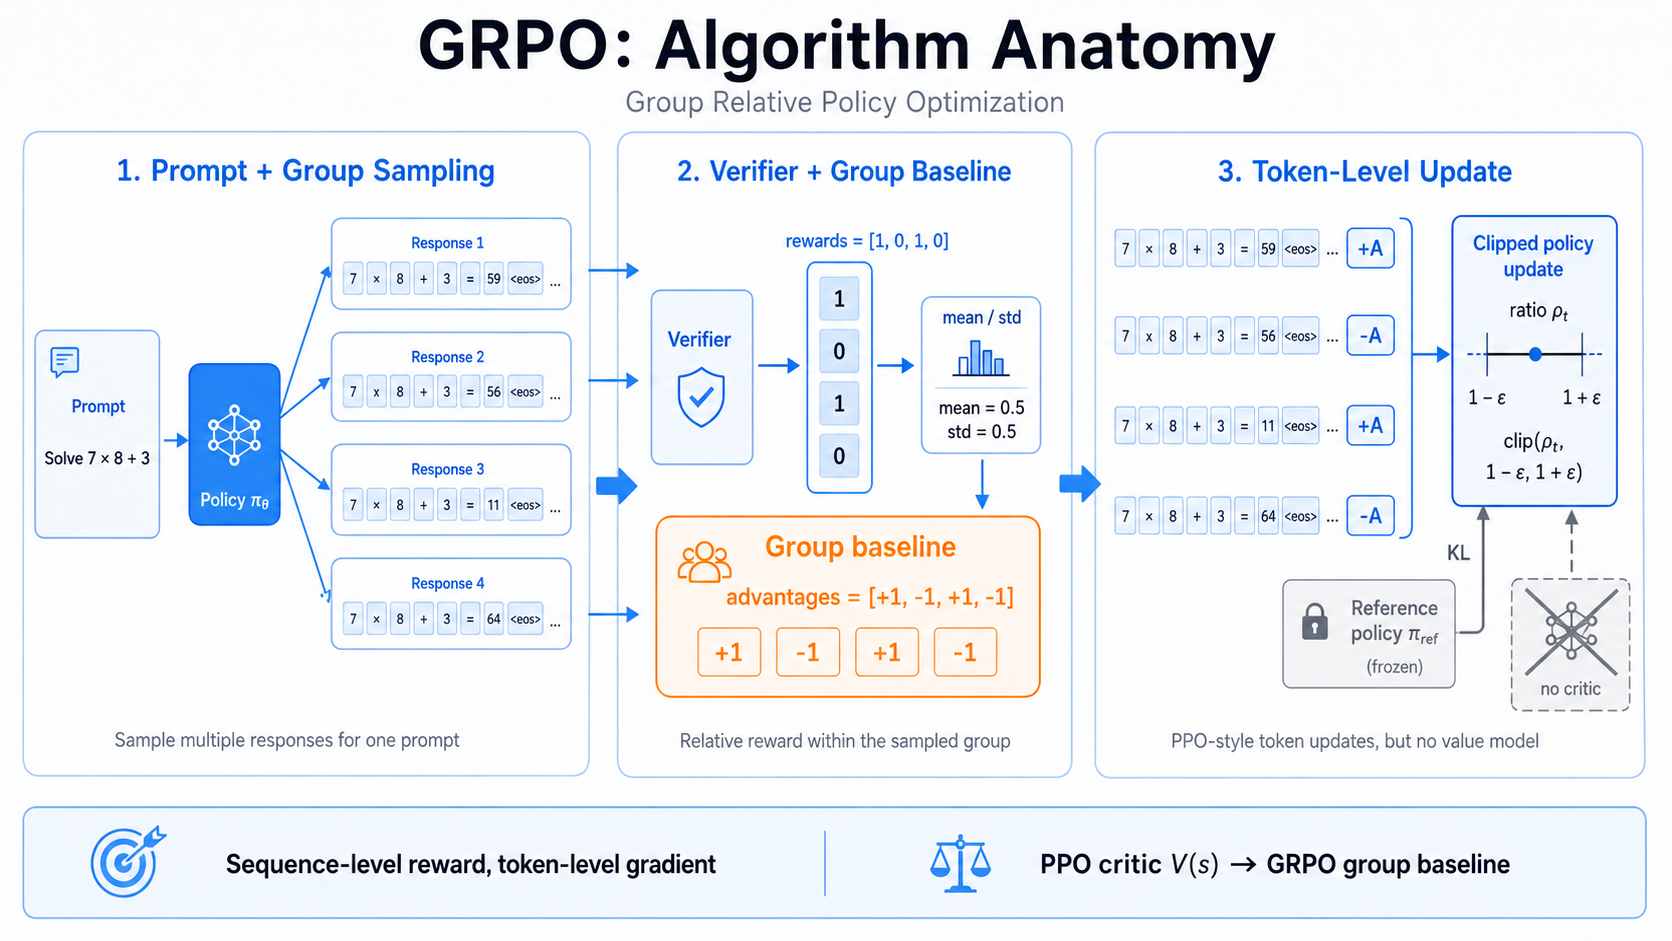
\includegraphics[width=0.95\textwidth]{figures/ch16/fig_grpo_step.png}
\caption{\textbf{One GRPO training step.} For each prompt, sample a group of responses, score each response with a verifier, normalize rewards within the group, and apply a PPO-style token-level clipped update. The learned value model from PPO is replaced by a group baseline, which is why GRPO is critic-free.}
\label{fig:grpo-step}
\end{figure}

\subsection{Why the Group Baseline Works}

The group baseline is useful when prompts vary in difficulty. Suppose your batch contains one easy algebra problem and one hard olympiad problem. On the easy problem, most responses may be correct; on the hard problem, most responses may fail. Raw rewards $0/1$ do not distinguish ``correct on an easy prompt'' from ``correct on a hard prompt.'' Group normalization makes the comparison local to the prompt. A correct answer among mostly incorrect attempts receives a large positive advantage. A correct answer among many correct attempts receives a smaller advantage.

This is the critic-free counterpart to the value model in Chapter~\ref{ch:rl-foundations}. PPO asks a learned critic: ``How good is this partial sequence compared to expectation?'' GRPO asks the group: ``How good is this response compared to the other attempts on the same prompt?'' In the race-timing analogy, PPO keeps a coach who predicts your lap time at every checkpoint; GRPO simply compares your actual finish time to the other drivers' times on the same track.

\noindent\fbox{\parbox{\dimexpr\textwidth-2\fboxsep-2\fboxrule\relax}{%
\textbf{Pause and verify.}\quad Your 3B model samples $G=4$ responses to the same math prompt. Verifier rewards are $[1,0,1,0]$. The group mean is $\bar{r}=0.5$ and the standard deviation is $0.5$, so the advantages are $[+1,-1,+1,-1]$. Now suppose rewards are $[1,1,1,0]$. The mean is $0.75$ and the standard deviation is about $0.43$, so the correct responses get advantages around $+0.58$ and the failed response gets about $-1.73$. \emph{The single failure becomes highly informative because it is worse than the group on the same prompt.}
}}

\begin{tcolorbox}[colback=blue!5, colframe=blue!40, title=\textbf{Worked Example: One GRPO Step on Math}]
\textbf{Prompt}: ``What is $7 \times 8 + 3$?''

\textbf{Step 1: Sample.} Your 3B model generates $G=4$ responses at temperature 0.8:

\begin{itemize}[nosep]
  \item $y_1$: ``Let me compute: $7 \times 8 = 56$, then $56 + 3 = 59$. The answer is $\backslash$boxed\{59\}.'' (correct)
  \item $y_2$: ``$7 \times 8 = 54$, $54 + 3 = 57$. $\backslash$boxed\{57\}.'' (wrong)
  \item $y_3$: ``First, $7 \times 8$. I know $7 \times 7 = 49$, so $7 \times 8 = 49 + 7 = 56$. Then $56 + 3 = 59$. $\backslash$boxed\{59\}.'' (correct)
  \item $y_4$: ``The answer is $\backslash$boxed\{59\}.'' (correct but no reasoning)
\end{itemize}

\textbf{Step 2: Verify.} The verifier extracts boxed answers and compares to ground truth 59. Rewards: $r = [1, 0, 1, 1]$.

\textbf{Step 3: Normalize.} Group mean $\bar{r} = 0.75$, $\sigma_r \approx 0.43$. Advantages: $\hat{A} \approx [+0.58, -1.73, +0.58, +0.58]$. Response $y_2$ receives a large negative advantage.

\textbf{Step 4: Update.} For each token $t$ in each response, compute $\rho_{i,t}$ and apply the clipped objective with $\hat{A}_i$. All tokens in $y_2$ are pushed down. All tokens in $y_1, y_3, y_4$ are pushed up---including $y_4$'s shortcut, which the model may later learn is fragile on harder problems.

\textbf{Step 5: KL check.} Compute KL divergence between $\pi_\theta$ and $\pi_{\text{ref}}$. If KL exceeds target, increase $\beta$.
\end{tcolorbox}

\subsection{Operational Details}

GRPO reduces memory by removing the value model, but it increases rollout demand: you now sample multiple responses per prompt. If $G=8$ and each response is 1{,}000 tokens, one prompt produces 8{,}000 generated tokens before any gradient update. As in Chapter~\ref{ch:rlhf}, rollout generation often dominates wall-clock time.

\subsubsection*{Memory: PPO vs GRPO}

Chapter~\ref{ch:rlhf} warned that PPO-RLHF requires four model-sized objects: policy, reference, reward model, and value model. For a 7B model in bf16, that is at least 56~GB in model weights alone, before activations and optimizer state. GRPO removes the value model entirely and, in settings where the verifier is a script rather than a neural network, also removes the reward model. A 7B GRPO setup with a script verifier needs only two model-sized objects (policy + reference), cutting the model-weight floor roughly in half. With QLoRA (Chapter~\ref{ch:peft}), the reference can share the quantized base with the policy adapter. This is why GRPO has become a common choice for low-resource open-source reasoning RL, alongside PPO-style RLVR, rejection/self-training loops, and newer GRPO variants.

\subsubsection*{Typical Hyperparameters}

\begin{center}
\small
\begin{tabularx}{\textwidth}{@{}l l X@{}}
\toprule
\textbf{Hyperparameter} & \textbf{Typical range} & \textbf{Notes} \\
\midrule
Group size $G$ & 4--16 & Larger $G$ gives better baseline estimates but more rollout cost \\
Sampling temperature & 0.7--1.0 & Too low reduces group diversity; too high wastes compute on incoherent samples \\
Clip $\epsilon_{\text{clip}}$ & 0.1--0.2 & Same role as PPO clipping; unrelated to $\epsilon_{\text{std}}$ in reward normalization \\
KL coefficient $\beta$ & 0.01--0.1 & Often lower than RLHF because the main reward is not a learned preference proxy \\
Learning rate & $5 \times 10^{-7}$ to $2 \times 10^{-6}$ & Smaller than SFT; comparable to RLHF \\
PPO epochs per batch & 1--2 & Conservative; GRPO groups are more informative than single-response batches \\
Max response length & 2{,}048--8{,}192 & Reasoning models need headroom for long chains of thought \\
\bottomrule
\end{tabularx}
\normalsize
\end{center}

\subsubsection*{Implementation Pitfalls}

Three details matter in code. First, the length normalization in Equation~\ref{eq:grpo-loss} is a design choice, not a law of nature. Normalizing by $|y_i|$ keeps long responses from producing larger total gradients simply because they contain more tokens, but it can also dilute the learning signal for useful long reasoning. Later RLVR variants such as DAPO explicitly revisit this normalization and related clipping choices to reduce length bias and improve training stability~\cite{yu2025dapo}. This is why response length should be a training metric, not just a generation setting: if solve rate improves only by making every answer much longer, you have learned a costly policy that may not be the one you want to deploy.

Second, the frozen reference policy can become stale during long runs. Early in training, KL to $\pi_{\text{ref}}$ is a useful measure of how far the policy has moved from the starting point. Late in training, the policy may be far enough away that the reference is more of an anchor than a fine-grained guide. Some production systems periodically refresh the reference or use staged training to avoid a single outdated anchor dominating the run.

Third, reward variance within groups falls as the model improves. If a prompt becomes all-pass, the group baseline no longer produces useful advantages; if it remains all-fail, there is no successful trajectory to reinforce. Curriculum refresh is therefore part of the algorithm, not a data-cleaning afterthought.

The practical dashboard is therefore different from a standard SFT run. You monitor held-out solve rate, average response length, invalid-format rate, KL to reference, reward variance within group, and rollout throughput. If solve rate rises while invalid formats rise, the verifier contract is being exploited. If length rises while solve rate stalls, the model is spending tokens without buying accuracy. If reward variance collapses, the curriculum has drifted out of the useful difficulty band.

\begin{figure}[t]
\centering
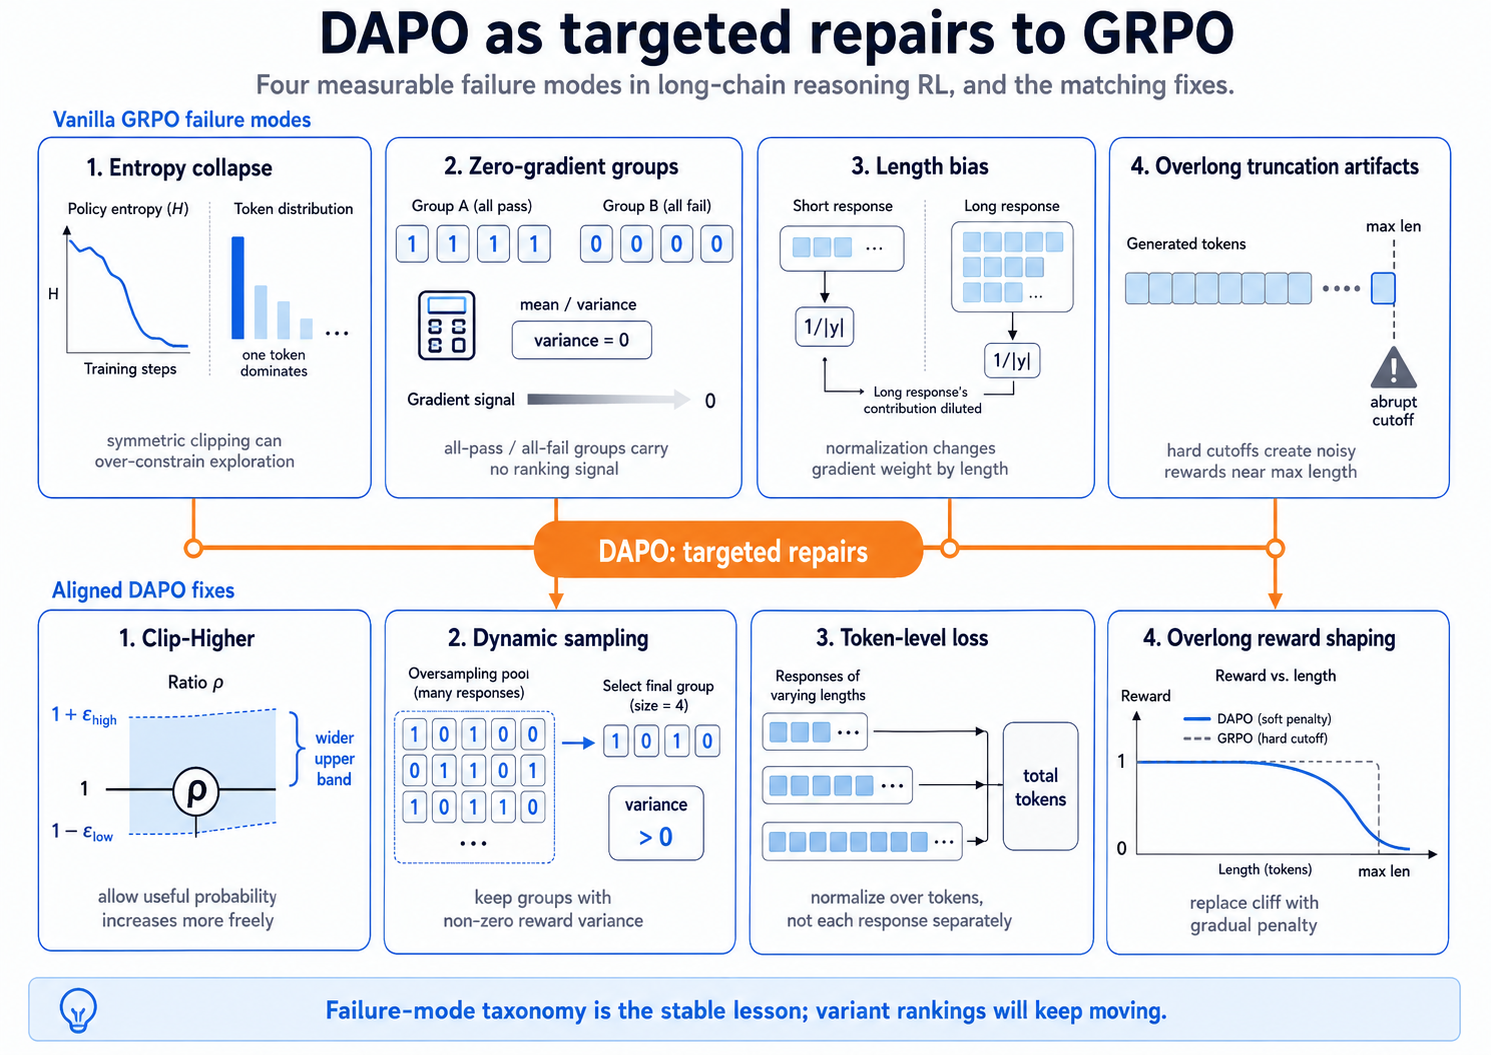
\includegraphics[width=0.95\textwidth]{figures/ch16/fig_dapo_failure_modes.png}
\caption{\textbf{DAPO as targeted repairs to vanilla GRPO.} Vanilla GRPO exposes several practical failure modes in long-chain reasoning: entropy collapse, zero-gradient groups, length bias, and overlong truncation artifacts. DAPO addresses them with asymmetric clipping, dynamic sampling, token-level loss normalization, and overlong reward shaping. The durable lesson is the failure-mode taxonomy, not a frozen variant ranking.}
\label{fig:dapo-failure-modes}
\end{figure}

For Project~3, a practical starting point is:

\begin{tcolorbox}[colback=orange!5, colframe=orange!60, title=\textbf{For Project~3: A GRPO Starting Recipe}]
\begin{itemize}[nosep]
  \item \textbf{Group size}: $G=4$ for a 3B model on limited hardware; increase to $G=8$ if rollout throughput allows.
  \item \textbf{Rewards}: binary correctness plus a small format reward. Keep auxiliary rewards small enough that correctness dominates.
  \item \textbf{Sampling}: temperature $0.7$--$1.0$ to produce diverse attempts; too-low temperature gives uninformative groups.
  \item \textbf{KL}: keep a reference policy and monitor KL. Verifiable reward does not make KL irrelevant.
  \item \textbf{Metrics}: held-out solve rate, average response length, fraction of invalid formats, KL to reference, and reward variance within group.
\end{itemize}
\end{tcolorbox}

\subsection{PPO vs GRPO: What Actually Changed}

GRPO is easiest to understand as a surgical modification to PPO. It keeps the token-level policy update, clipping, KL regularization, and rollout policy from Chapter~\ref{ch:rl-foundations}. It removes the learned value model and replaces its advantage estimate with a group-relative baseline.

\begin{center}
\small
\begin{tabularx}{\textwidth}{@{}lXX@{}}
\toprule
\textbf{Component} & \textbf{PPO for RLHF} & \textbf{GRPO for Reasoning RL} \\
\midrule
Advantage estimate & GAE with learned value model $V_\psi$ & Group-normalized verifier rewards \\
Critic / value model & Required; usually model-sized & Not used \\
Per-prompt samples & Often one or a few responses per prompt & Group of $G$ responses for the same prompt \\
Reward source & Learned RM plus KL penalty & Verifier / rubric plus KL penalty \\
Reward granularity & Terminal RM score plus per-token KL & Sequence-level verifier reward broadcast to tokens \\
Clipping & Per-token ratio clipping & Per-token ratio clipping \\
Memory floor & Policy + reference + RM + value model & Policy + reference; verifier may be a script \\
Main cost & Rollout + four model-sized objects & Rollout volume from group sampling \\
\bottomrule
\end{tabularx}
\normalsize
\end{center}

This table is the core algorithmic contrast. GRPO is not ``PPO but for math''; it is PPO with the critic replaced by a within-prompt race. The race timing system supplies the outcome, and the other runners on the same track supply the baseline. R1-Zero is the public anchor for this design pattern: GRPO-style training with rule-based math rewards, no learned value model, and no supervised cold-start for reasoning traces. The simplicity of the algorithm is part of the lesson---the power came from the verifier and the scale of training, not from a more complex optimizer.

\subsection{KL in Reasoning RL}

The KL term in Equation~\ref{eq:grpo-loss} looks familiar from Chapters~\ref{ch:preference-learning}--\ref{ch:rlhf}, but its job changes. In RLHF, KL has three roles: it regularizes a learned reward model, preserves base capabilities, and prevents diversity collapse. The first role is less central in verifier-based reasoning RL. A math checker or unit-test suite does not become unreliable merely because the policy leaves the SFT distribution; it checks the final answer or executes the code.

That does not make KL optional. Reasoning RL can still degrade general instruction-following ability, collapse into one verbose reasoning template, or exploit verifier-specific formats. KL mainly preserves the useful base distribution and slows runaway style drift. This is why reasoning-RL runs often tolerate smaller $\beta$ than RLHF runs with learned reward models, but still monitor KL closely. The reward is more reliable; the policy can still become worse outside the checked task.

\subsection{The Algorithm--Reward Taxonomy}

GRPO is a representative implementation, not the definition of reasoning RL. The broader design space has two axes: the optimization algorithm and the reward source.

\begin{figure}[t]
\centering
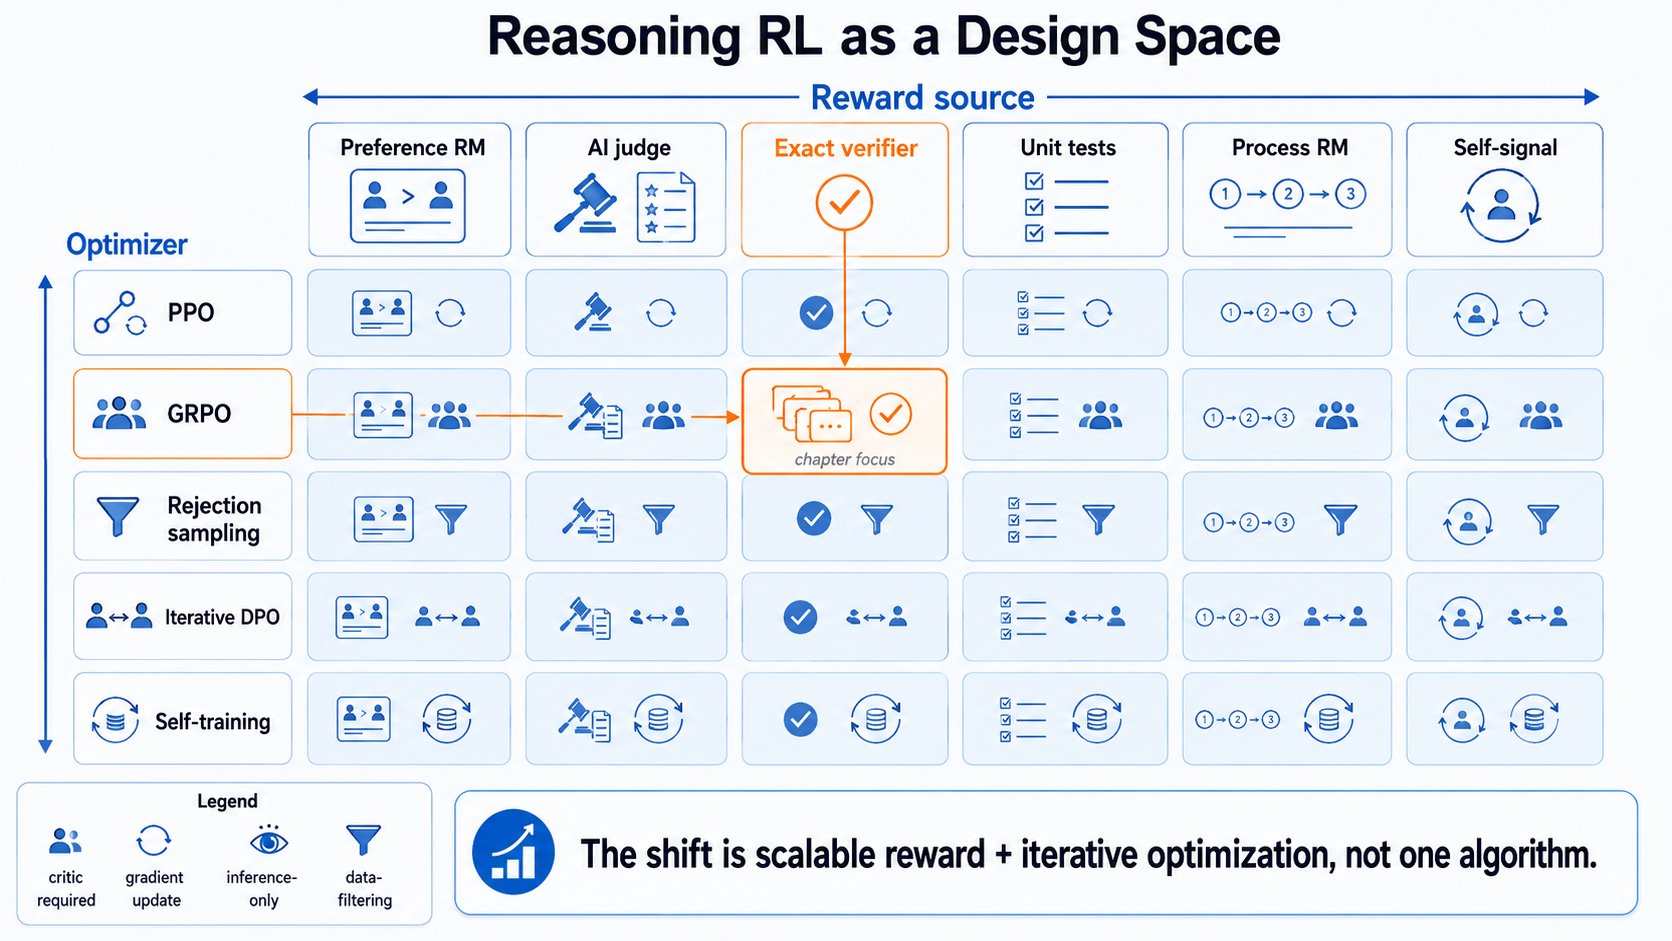
\includegraphics[width=0.95\textwidth]{figures/ch16/fig_algorithm_reward_taxonomy.png}
\caption{\textbf{Reasoning RL is an algorithm--reward design space.} The reward source can be a human preference model, an AI preference model, an exact verifier, a unit-test suite, a process reward model, or a self-generated signal. The optimizer can be PPO, GRPO, rejection sampling, iterative DPO, or self-training. The 2024--2026 shift is not a single algorithm; it is the pairing of scalable reward sources with iterative optimization.}
\label{fig:algorithm-reward-taxonomy}
\end{figure}

\begin{center}
\small
\begin{tabularx}{\textwidth}{@{}lXXX@{}}
\toprule
\textbf{Method} & \textbf{Reward source} & \textbf{Critic?} & \textbf{Typical domain} \\
\midrule
PPO-RLHF & Learned human preference RM & Yes & Chat alignment, safety, style \\
PPO-RLVR & Verifier or unit tests & Yes & Math, code, formal tasks \\
GRPO & Verifier / binary reward / rubric & No & Reasoning RL, low-resource setups \\
Rejection sampling & Verifier or RM ranker & No gradient & Best-of-$N$, data filtering \\
Iterative DPO & Pairwise preferences from fresh samples & No critic & Preference refinement, offline/online hybrids \\
Self-training / ReST & Model-generated samples filtered by reward & No explicit RL step & Reasoning traces, translation, summarization \\
\bottomrule
\end{tabularx}
\normalsize
\end{center}

\begin{figure}[t]
\centering
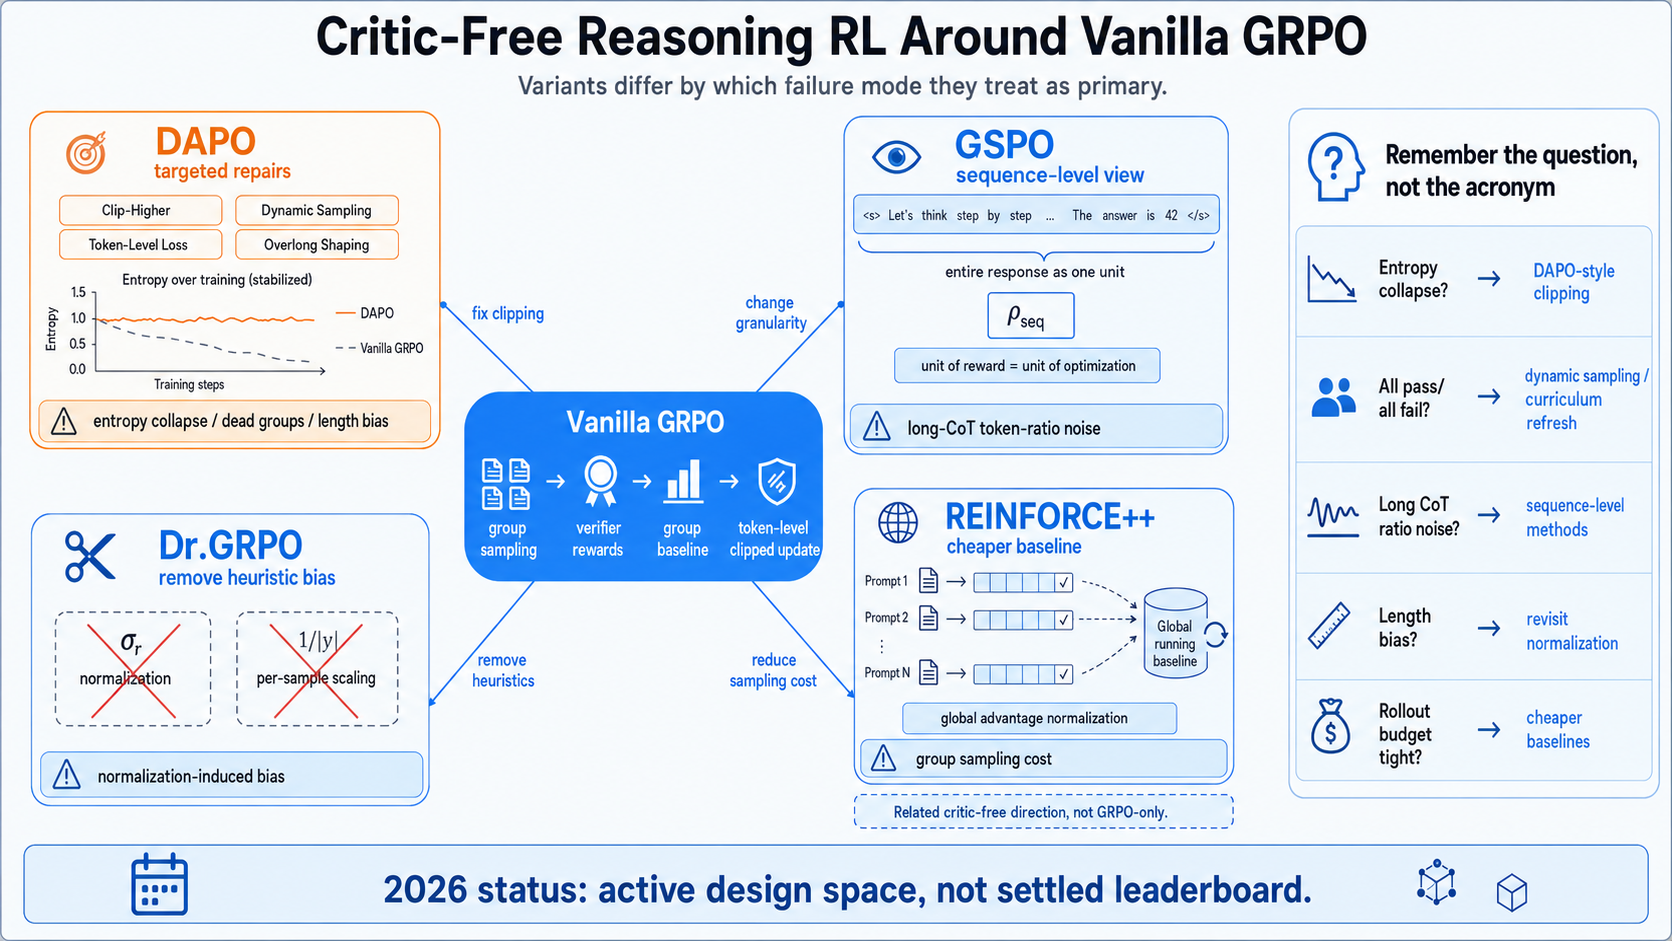
\includegraphics[width=0.95\textwidth]{figures/ch16/fig_grpo_variants_landscape.png}
\caption{\textbf{GRPO variants as competing bets on the right abstraction level.} DAPO adds targeted fixes for vanilla GRPO pathologies, GSPO moves ratio logic toward the sequence level, Dr.GRPO removes heuristic normalizations, and REINFORCE++ simplifies the baseline. The field is moving quickly, so the durable question is which failure mode each variant is trying to solve.}
\label{fig:grpo-variants-landscape}
\end{figure}

\begin{quickrecap}
\textbf{Quick Recap.}
\begin{itemize}[nosep,leftmargin=1.5em]
  \item GRPO replaces PPO's learned value model with a group baseline computed from multiple samples for the same prompt.
  \item Rewards are sequence-level, but the clipped policy update is token-level.
  \item GRPO reduces memory but increases rollout volume because each prompt needs several sampled responses.
  \item KL still matters in reasoning RL, but less as reward-model regularization and more as capability and style preservation.
  \item Reasoning RL is a design space: optimizer $\times$ reward source, not just GRPO.
\end{itemize}
\textit{Next: should the reward score only the final answer, or the reasoning process itself?}
\end{quickrecap}


%----------------------------------------------------------------------
\section{Process vs Outcome Rewards}
\label{sec:process-outcome}

Outcome rewards judge the final answer. Process rewards judge intermediate reasoning steps. The distinction matters because reasoning is not just a final token; it is a trajectory. In the race-timing analogy, outcome reward is the finish-line clock: did you complete the lap within the time limit? Process reward is the sector-by-sector split: how fast were you through each turn? The clock tells you whether you won; the sector splits tell you where you lost time.

\subsection{Outcome Reward Models}

An \textbf{outcome reward model} (ORM) or outcome verifier scores the completed response. It asks: did the final answer pass? This is cheap and scalable. Math answer checkers and unit tests are outcome rewards. The downside is credit assignment. If a 1{,}500-token solution ends with the wrong answer, the outcome reward says ``fail'' but does not identify which step went wrong.

Outcome rewards work surprisingly well when the model can discover useful reasoning patterns from many attempts. This is the DeepSeek-R1 lesson: with enough sampling, a verifier, and a stable optimizer, trajectory-level reward can induce long reasoning behaviors. But outcome reward is blunt. It can reward lucky answers and punish mostly-correct reasoning with one arithmetic slip.

\subsection{Process Reward Models}

A \textbf{process reward model} (PRM) scores steps. Lightman et al.\ showed that supervising the reasoning process can outperform supervising only final outcomes on hard math problems, and released PRM800K, a dataset of step-level labels~\cite{lightman2023verify}. A PRM can be used in several ways:

\begin{itemize}[nosep]
  \item \textbf{Training reward}: add step-level rewards during RL so the model receives denser feedback.
  \item \textbf{Search evaluator}: use the PRM to rank partial reasoning paths during best-of-$N$ or tree search.
  \item \textbf{Data filter}: keep reasoning traces whose intermediate steps look valid.
\end{itemize}

The cost is annotation and specification. Step-level labels are expensive. They may also encode a style of reasoning rather than correctness itself. A PRM trained on human-labeled steps can become another learned proxy, bringing back some of the RLHF problems Chapter~\ref{ch:rlhf} warned about.

The evidence is strongest when the task is hard enough that final-answer reward is too sparse. Lightman et al.\ found that process supervision outperformed outcome supervision most clearly on the hardest MATH problems, where many wrong solutions share a long correct prefix before diverging at a critical step~\cite{lightman2023verify}. The PRM could identify the divergence point; the ORM could only say ``wrong.'' On easier problems, or with stronger base models, the gap narrows: if many sampled solutions already reach the correct answer, the cheap outcome signal may be enough. Later work has shown that the PRM advantage is task- and scale-dependent---stronger models with more sampling can compensate for the lack of step-level feedback. This is the practical rule: use process reward when credit assignment, not reward availability, is the bottleneck.

\begin{figure}[t]
\centering
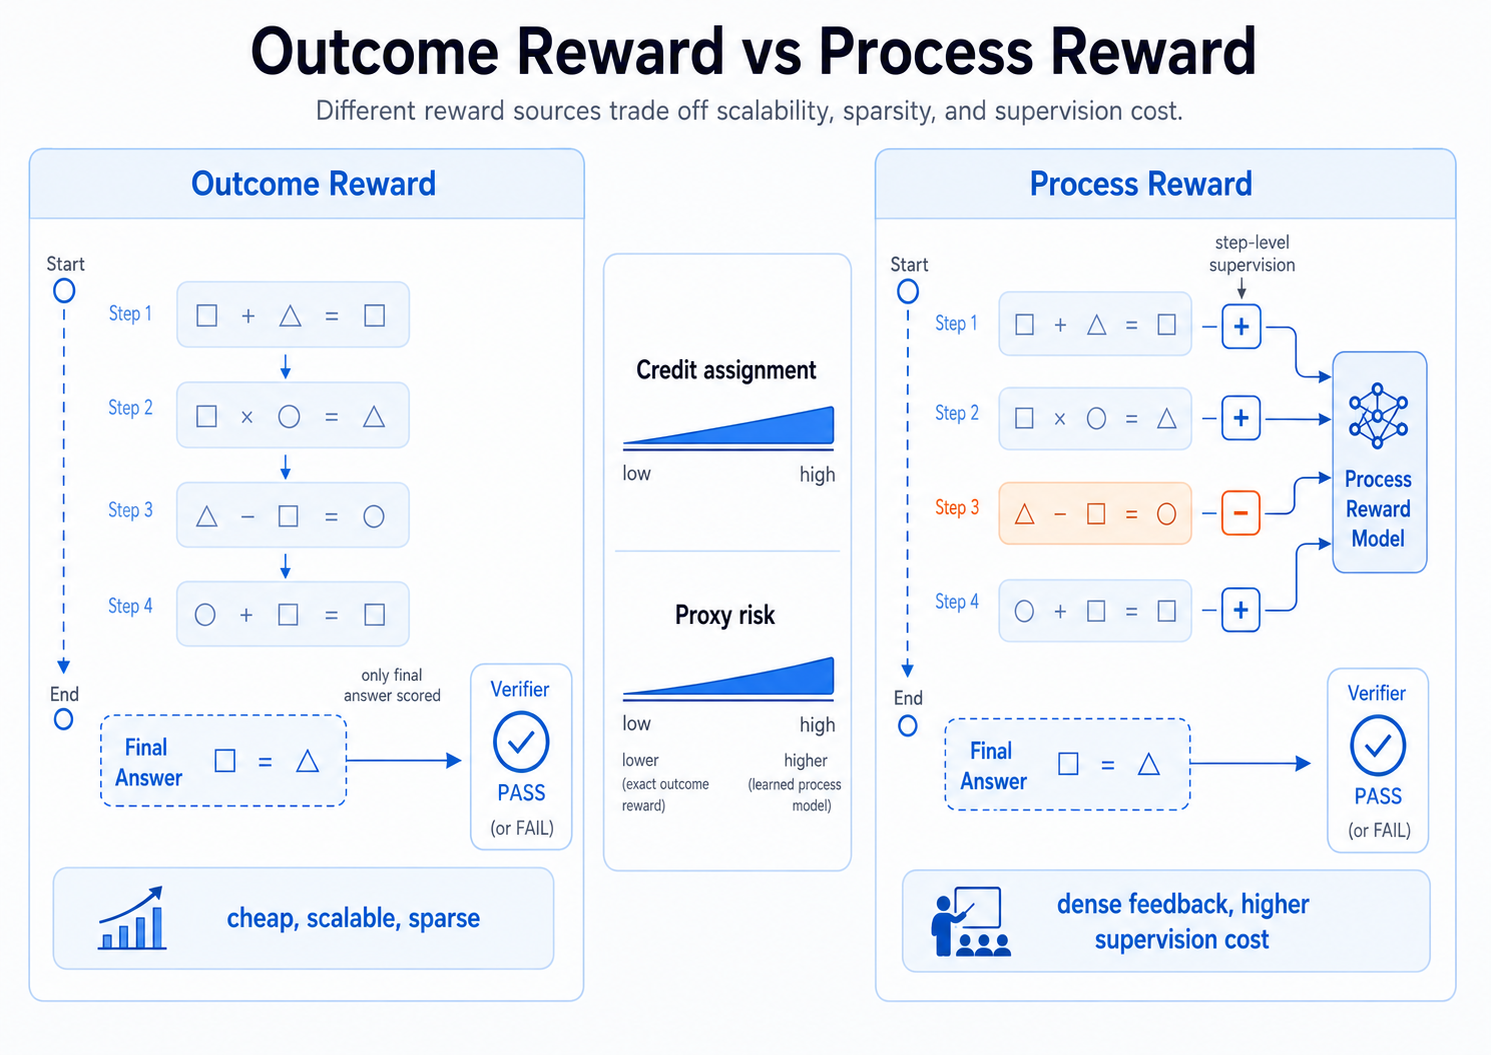
\includegraphics[width=0.95\textwidth]{figures/ch16/fig_process_vs_outcome.png}
\caption{\textbf{Outcome rewards vs process rewards.} Outcome rewards score only the final response: correct answer, passed tests, accepted proof. Process rewards score intermediate reasoning steps, providing denser credit assignment but requiring more supervision and introducing another learned proxy.}
\label{fig:process-vs-outcome}
\end{figure}

\subsection{Current Practical Consensus}

For many scalable systems, outcome reward is the usual starting point because it is cheap. Process reward is useful when:

\begin{itemize}[nosep]
  \item final-answer reward is too sparse;
  \item many wrong solutions share a long correct prefix;
  \item search over intermediate reasoning paths is part of inference;
  \item the domain can support reliable step-level labels or formal checking.
\end{itemize}

The safe summary is: outcome reward scales; process reward guides. Reasoning RL often starts with outcome reward and adds process signals only where the sparse signal is not enough.

\begin{tcolorbox}[colback=orange!5, colframe=orange!60, title=\textbf{For Project~3: Choosing Your Reward Signal}]
\begin{itemize}[nosep]
  \item \textbf{Start with outcome reward}. For math, binary answer correctness is the simplest and most reliable signal. Do not add process rewards until you have a working outcome-reward baseline.
  \item \textbf{Add format reward conservatively}. A small bonus for producing a \texttt{\textbackslash boxed\{\}} answer helps the verifier extract the answer, but keep the coefficient small (0.1--0.2$\times$ the correctness reward) so the model does not learn to produce valid format with wrong answers.
  \item \textbf{Monitor reward composition}. Track what fraction of total reward comes from correctness vs auxiliary signals. If auxiliary rewards dominate, the model is optimizing the wrong thing.
  \item \textbf{Do not build a PRM for Project~3}. Step-level labels require either human annotation or a strong teacher model. At 3B scale with limited data, outcome reward plus auxiliary format reward is the right starting point.
\end{itemize}
\end{tcolorbox}

\begin{quickrecap}
\textbf{Quick Recap.}
\begin{itemize}[nosep,leftmargin=1.5em]
  \item Outcome rewards are cheap and scalable but provide weak credit assignment.
  \item Process rewards provide denser feedback but require step-level supervision or a learned proxy.
  \item PRMs are useful for training, search, and data filtering, but they reintroduce proxy-risk.
\end{itemize}
\textit{Next: what behaviors emerge when models train against these rewards?}
\end{quickrecap}


%----------------------------------------------------------------------
\section{Emergent Reasoning Behaviors from RL}
\label{sec:emergent-reasoning}

The most interesting claim about reasoning RL is not that it improves benchmark scores. It is that optimizing outcome reward can change the \emph{style} of generation. Models learn to spend more tokens on hard problems, check their own work, backtrack from dead ends, and revise plans. These behaviors are not necessarily copied from demonstrations. They can be reinforced because they correlate with success.

\subsection{Longer Deliberation}

In SFT, reasoning length is inherited from the demonstration data. If the dataset contains short solutions, the model imitates short solutions. In RL with a verifier, length becomes an instrumental variable: if thinking longer helps solve harder problems, longer traces receive higher reward. If extra length does not help, KL and length penalties can keep it under control.

This is the training-time version of the test-time observation from Chapter~\ref{ch:evaluation}: reasoning models benefit from spending more compute on hard problems. RL teaches the policy when that extra computation is useful.

\subsection{Self-Correction and Backtracking}

Self-correction becomes useful when mistakes are recoverable. Suppose a model starts a solution, notices a contradiction, and restarts with a different approach. A pure imitation objective may treat the detour as inefficient. A verifier only sees the final success. If self-correction increases success probability, RL reinforces the entire trajectory, including the correction behavior.

The same logic applies to backtracking in code. A model writes an implementation, mentally tests an edge case, realizes it fails, and rewrites the function. If the final code passes tests, the trajectory receives positive reward. Over many attempts, the model can learn that checking edge cases before finalizing is useful.

\subsection{Reading the Training Log}

How do you know these behaviors are emerging during training? You cannot inspect every generated trajectory. But you can watch aggregate metrics:

\begin{itemize}[nosep]
  \item \textbf{Average response length} increases on hard prompts but not on easy prompts---the model is learning to spend more tokens where it helps.
  \item \textbf{Held-out solve rate} improves on problems the training distribution does not include---the model is generalizing, not memorizing answers.
  \item \textbf{Correction frequency} rises when traces include phrases like ``wait,'' ``let me reconsider,'' or ``that's wrong.'' This is not conclusive evidence of true self-correction, but it tracks with solve-rate improvement.
  \item \textbf{Reward variance within groups} decreases over training on easy prompts (the model solves them reliably) but stays high on hard prompts (still exploring).
\end{itemize}

These are diagnostic signals, not proofs. A model that produces longer outputs may just be verbose. A model that writes ``let me check'' may not actually check. The verifier is the ground truth: if solve rate is climbing on held-out problems, the training is working regardless of what the traces look like.

\subsection{Case Study: DeepSeek-R1-Zero}

R1-Zero is the cleanest public demonstration of this chapter's thesis. It was not the final user-facing R1 recipe. It was the ablation that asked a sharper question: what happens if a strong base model is trained directly with large-scale RL from rule-based rewards, without first imitating human-written reasoning traces?

The answer was not merely a higher benchmark score. DeepSeek reported that R1-Zero developed longer reasoning traces, self-verification, reflection-like phrases, and backtracking during RL training~\cite{deepseekai2025r1}. Three empirical observations from the paper are worth remembering:

\begin{enumerate}[nosep]
  \item \textbf{Response length trajectory.} The average response length grew substantially over training. The model learned to spend more tokens on hard problems because longer deliberation correlated with verifier success. This is the training-log signature of emergent reasoning: the policy discovers that thinking longer helps, not because demonstrations showed long traces, but because longer traces passed the verifier more often.
  \item \textbf{The ``aha moment.''} At a certain point during training, the model began producing self-correction phrases---pausing mid-solution, reconsidering an earlier step, and reallocating effort. The paper highlights this as evidence that RL can induce metacognitive-like behaviors from outcome reward alone. Whether the model is ``truly'' reflecting or merely producing tokens that correlate with success is an open question, but the behavioral change is real and measurable.
  \item \textbf{R1-Zero vs R1.} R1-Zero demonstrated that verifiable reward can surface reasoning behavior without supervised reasoning traces. R1 then added cold-start SFT data for readability and format, additional RL stages, and distillation into smaller models. The lesson is not ``SFT is unnecessary.'' The lesson is that verifier-based RL can supply a signal strong enough to change the model's generation strategy, and production-quality models still benefit from supervised data and multi-stage refinement on top.
\end{enumerate}

This case study also sets a boundary on what this chapter can claim. R1-Zero is evidence that outcome-reward RL can induce useful reasoning behaviors in a strong base model. It is not evidence that every base model can be turned into a reasoning model by adding a verifier. The base model still needs latent mathematical and linguistic capability; the verifier supplies selection pressure, not the capability itself.

\subsection{A Caution: Behavior vs Capability}

Do not over-interpret the word ``emergent.'' RL can amplify behaviors the base model already has in weak form. Chapter~\ref{ch:instruction-tuning} made this point for instruction following, and Chapter~\ref{ch:peft} made the mathematical version with low-dimensional fine-tuning. Reasoning RL often surfaces and strengthens latent reasoning patterns rather than creating reasoning from nothing.

\begin{tcolorbox}[colback=gray!8, colframe=gray!40]
\textbf{Echo: surfacing vs creating.} Chapter~\ref{ch:instruction-tuning} argued that SFT surfaces assistant behavior already made possible by pretraining. Chapter~\ref{ch:peft} argued that fine-tuning moves through a small subspace. Reasoning RL is the same theme with a stronger signal: a verifier repeatedly selects trajectories that solve the task. The model is still constrained by the capabilities pretraining gave it, but the optimization pressure is now aimed at outcomes rather than demonstrations.
\end{tcolorbox}

\begin{figure}[t]
\centering
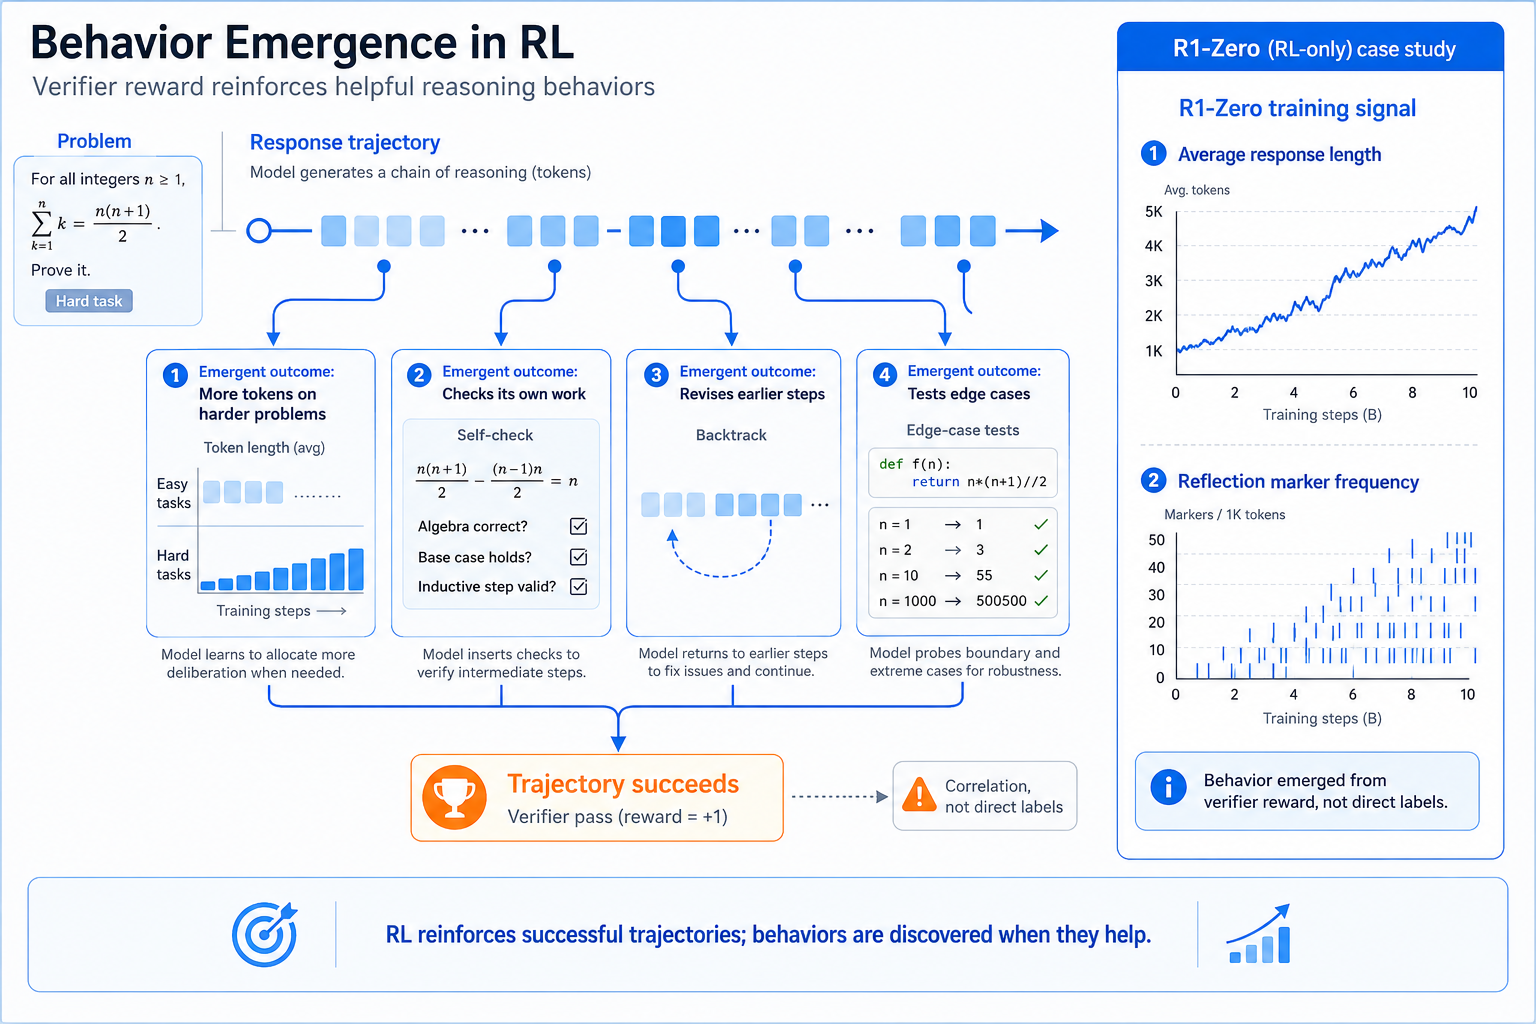
\includegraphics[width=0.95\textwidth]{figures/ch16/fig_emergent_behaviors.png}
\caption{\textbf{Reasoning behaviors reinforced by verifier reward.} Longer deliberation, self-checking, backtracking, and edge-case testing can emerge because they correlate with verifier success. RL does not need to label each behavior explicitly; it reinforces trajectories that solve the task.}
\label{fig:emergent-behaviors}
\end{figure}

\begin{quickrecap}
\textbf{Quick Recap.}
\begin{itemize}[nosep,leftmargin=1.5em]
  \item RL can reinforce long deliberation, self-correction, and backtracking when those behaviors improve verifier success.
  \item Diagnostic signals include response length on hard vs easy prompts, held-out solve rate, correction frequency, and within-group reward variance.
  \item RL surfaces and amplifies latent capabilities; it does not make the base model unlimited.
\end{itemize}
\textit{Next: what data infrastructure makes this training loop possible?}
\end{quickrecap}


%----------------------------------------------------------------------
\section{Reasoning Data Infrastructure}
\label{sec:reasoning-data}

Reasoning RL looks algorithmic, but its bottleneck is often data infrastructure. You need prompts with known answers, verifiers that work, sampling settings that produce diversity, and held-out evaluations that cannot be memorized. The reward may be cheap once built, but building the task distribution is not free.

\subsection{Problem Sources and Difficulty}

Math training requires problems at the right difficulty. If every prompt is too easy, all group rewards are $[1,1,1,1]$ and GRPO has little signal. If every prompt is too hard, rewards are $[0,0,0,0]$ and there is no positive trajectory to reinforce. The useful region is the frontier where the model sometimes succeeds and sometimes fails.

This is curriculum learning in practical form: keep the model near the edge of its competence. In the race-timing analogy, a training program that only includes straightforward highway laps (all-pass) or impossibly tight chicanes (all-fail) does not improve the driver. The useful training happens on tracks where the driver sometimes makes the turn and sometimes does not. A good reasoning dataset is not simply a collection of hard problems. It is a distribution that produces informative reward variance.

Concrete datasets make the scale visible. GSM8K contains about 8.5K grade-school math problems~\cite{cobbe2021gsm8k}. MATH contains about 12.5K competition-style problems across algebra, geometry, number theory, counting, and probability~\cite{hendrycks2021math}. Code training uses a different verifier stack: HumanEval-style function problems, MBPP-style programming tasks, APPS-style contest problems, and increasingly live benchmark suites that reduce contamination. The important point is not that one dataset is enough. It is that each dataset must come with a reliable checker and a held-out split that the training loop cannot memorize.

\paragraph{Difficulty filtering recipe.} A simple practical recipe is to estimate difficulty with the current policy. For each candidate problem, sample $N$ attempts and compute the empirical pass rate. Keep problems in a middle band, such as $0.1 \leq \text{pass@}N \leq 0.9$, and refresh the band as the model improves. Problems below the band are too hard to produce positive trajectories; problems above the band are too easy to produce contrast. This is the operational version of the ``frontier'' idea.

\subsection{Verifier Engineering}

Verifier engineering is the new data cleaning. For math, you need answer extraction, normalization, equivalence checking, and invalid-output handling. For code, you need sandboxing, timeout limits, hidden tests, and flaky-test detection. For formal proof, you need correct problem formalization and checker integration.

For Project~3, the math verifier can start with exact string matching only as a baseline. A more serious verifier normalizes fractions, decimals, signs, units, and equivalent symbolic expressions. SymPy-style equivalence checking helps, but it is not magic: expression parsing can fail, simplification can time out, and multiple valid forms may require task-specific rules. For code, the verifier should run in a sandbox, enforce CPU and memory limits, separate visible tests from hidden tests, and treat timeouts as failures. A weak verifier is not a small implementation detail; it is the reward function.

\begin{tcolorbox}[colback=orange!5, colframe=orange!60, title=\textbf{For Project~3: Building the Verifier}]
\begin{itemize}[nosep]
  \item \textbf{Start with answer extraction.} Decide where the final answer must appear, how invalid format is scored, and whether the model may include multiple candidate answers.
  \item \textbf{Normalize before comparing.} For math, handle fractions, decimals, signs, units, and equivalent symbolic expressions before declaring a response wrong.
  \item \textbf{Keep a hidden evaluation split.} Do not tune prompts, formatting rules, or auxiliary rewards against the same examples used to report solve rate.
  \item \textbf{Log verifier failures separately.} Track wrong answer, parse failure, timeout, invalid format, and verifier exception as different categories. A rising parse-failure rate means the model is learning around your reward interface.
  \item \textbf{Refresh difficulty.} Sample several attempts per problem and keep prompts whose pass rate is neither near zero nor near one.
\end{itemize}
\end{tcolorbox}

\noindent\fbox{\parbox{\dimexpr\textwidth-2\fboxsep-2\fboxrule\relax}{%
\textbf{Pause and verify.}\quad Your GRPO batch has 64 prompts, group size $G=4$, and binary rewards. On 40 prompts, all four responses fail. On 10 prompts, all four responses pass. On 14 prompts, the group has a mix of pass and fail. Which prompts produce useful group-relative learning signal? \emph{Mostly the 14 mixed prompts. All-pass and all-fail groups have near-zero reward variance, so normalized advantages vanish or become unstable. This is why difficulty scheduling is not cosmetic; it determines whether the algorithm has signal.}
}}

\subsection{Synthetic Reasoning Traces}

Many systems use synthetic reasoning traces: sample multiple solutions, keep the ones that verify, and fine-tune or train on them. STaR follows this pattern: generate rationales, keep successful ones, fine-tune, and repeat~\cite{zelikman2022star}. ReST generalizes the idea into a generate-filter-train loop~\cite{gulcehre2023rest}. These methods blur the boundary between RL and supervised learning. The reward filters data; the model learns from the filtered data.

\begin{figure}[t]
\centering
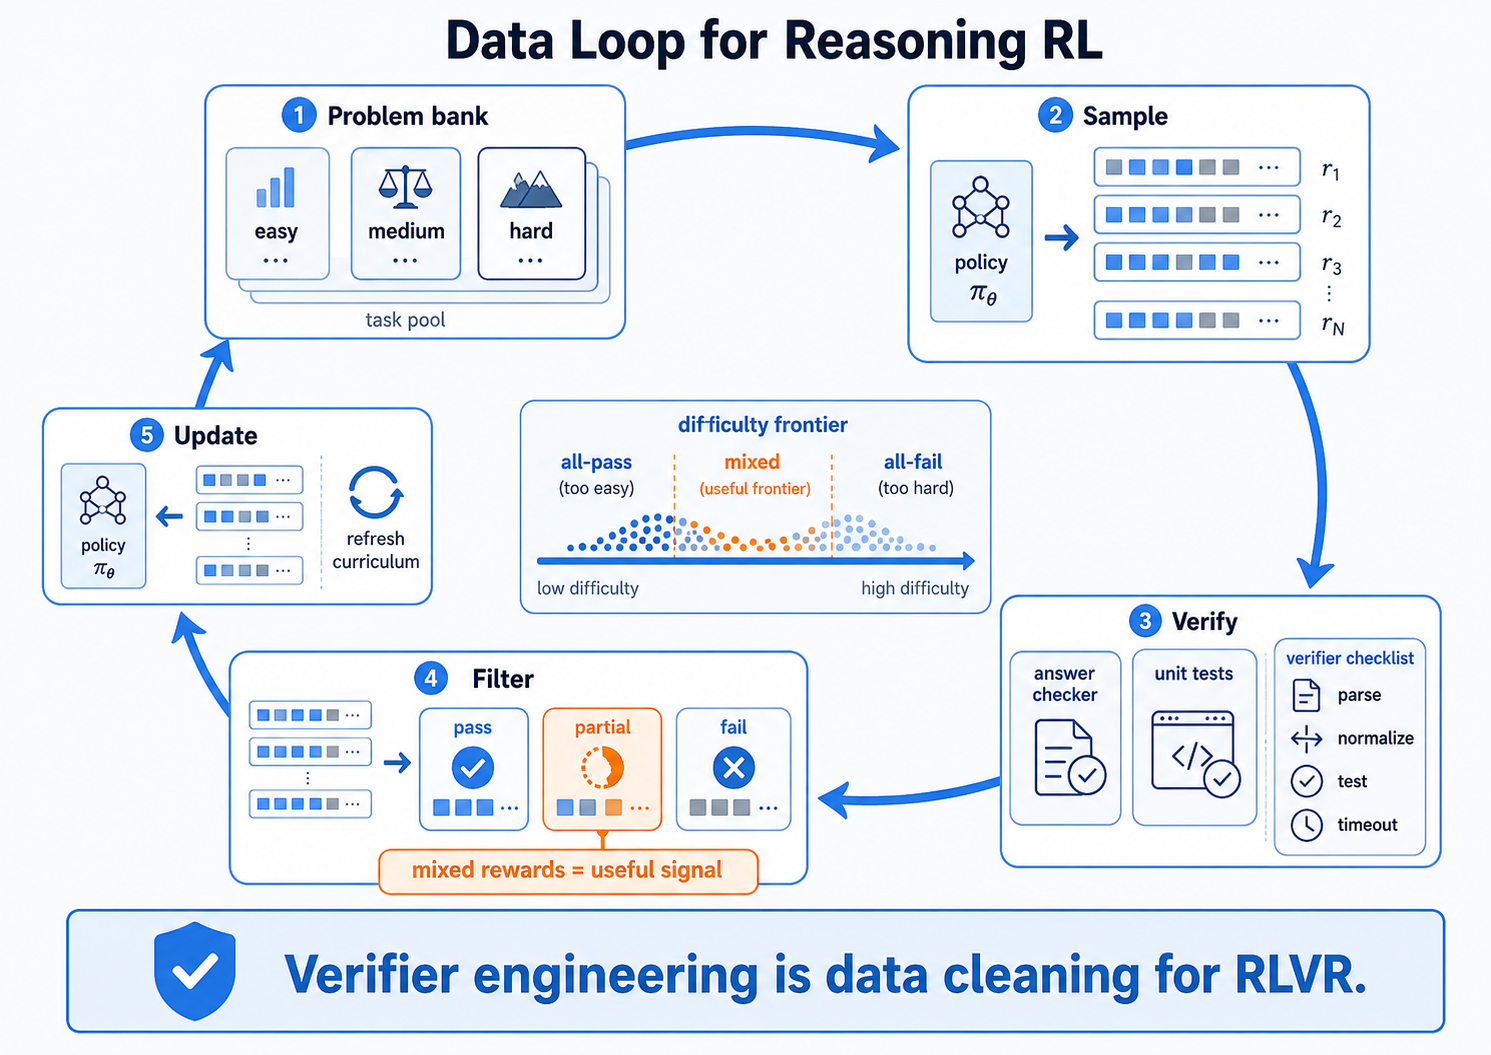
\includegraphics[width=0.95\textwidth]{figures/ch16/fig_reasoning_data_loop.png}
\caption{\textbf{Reasoning data infrastructure.} A reasoning-RL system is a loop: generate candidate problems or solutions, verify outputs, filter or score trajectories, update the policy, and refresh the curriculum. The algorithm is only as good as the task distribution and verifier pipeline.}
\label{fig:reasoning-data-loop}
\end{figure}

\begin{quickrecap}
\textbf{Quick Recap.}
\begin{itemize}[nosep,leftmargin=1.5em]
  \item Reasoning RL needs tasks near the model's frontier: neither all-pass nor all-fail.
  \item Verifier engineering is data cleaning for RLVR.
  \item Synthetic trace loops such as STaR and ReST use verifiers to turn model attempts into training data.
\end{itemize}
\textit{Next: why training-time reasoning connects directly to inference-time compute.}
\end{quickrecap}


%----------------------------------------------------------------------
\section{Inference-Time Scaling}
\label{sec:inference-scaling}

Chapters~\ref{ch:scaling-laws} and~\ref{ch:evaluation} introduced the idea that test-time compute is a third axis of capability. Pretraining scaling laws trade parameters against data. Reasoning models add another lever: generate more candidate reasoning paths, evaluate them, and select or aggregate.

\subsection{\texorpdfstring{Best-of-$N$}{Best-of-N} and Majority Voting}

The simplest inference-time scaling method is best-of-$N$: sample $N$ responses, score them with a verifier or reward model, and return the best. If the verifier is reliable, best-of-$N$ can improve accuracy without changing the model weights. Majority voting is similar: sample multiple solutions and choose the most common final answer. Self-consistency showed that voting across chain-of-thought samples improves reasoning accuracy~\cite{wang2022selfconsistency}.

These methods are expensive because they multiply generation cost by $N$. But they are easy to parallelize and require no gradient update. They are inference-time analogues of the group sampling used in GRPO: generate diverse attempts, use a reward or answer signal to decide which trajectories are useful. In the race-timing analogy, best-of-$N$ is running the lap $N$ times and reporting your best time. Majority voting is running it $N$ times and reporting the most common route. Neither changes the driver, but both improve the reported result.

\subsection{Search and Tree Methods}

For code and formal reasoning, search can be more structured. A model proposes partial programs, proof steps, or reasoning branches; a verifier or PRM scores intermediate states; the system expands promising branches. This begins to resemble classical search. The language model supplies proposals; the verifier supplies evaluation.

The boundary between training-time and inference-time compute is porous. A system can use search to solve problems, then add successful traces back into the training set. That is the same generate-filter-train loop from \S\ref{sec:reasoning-data}, now operating at inference scale.

\begin{figure}[t]
\centering
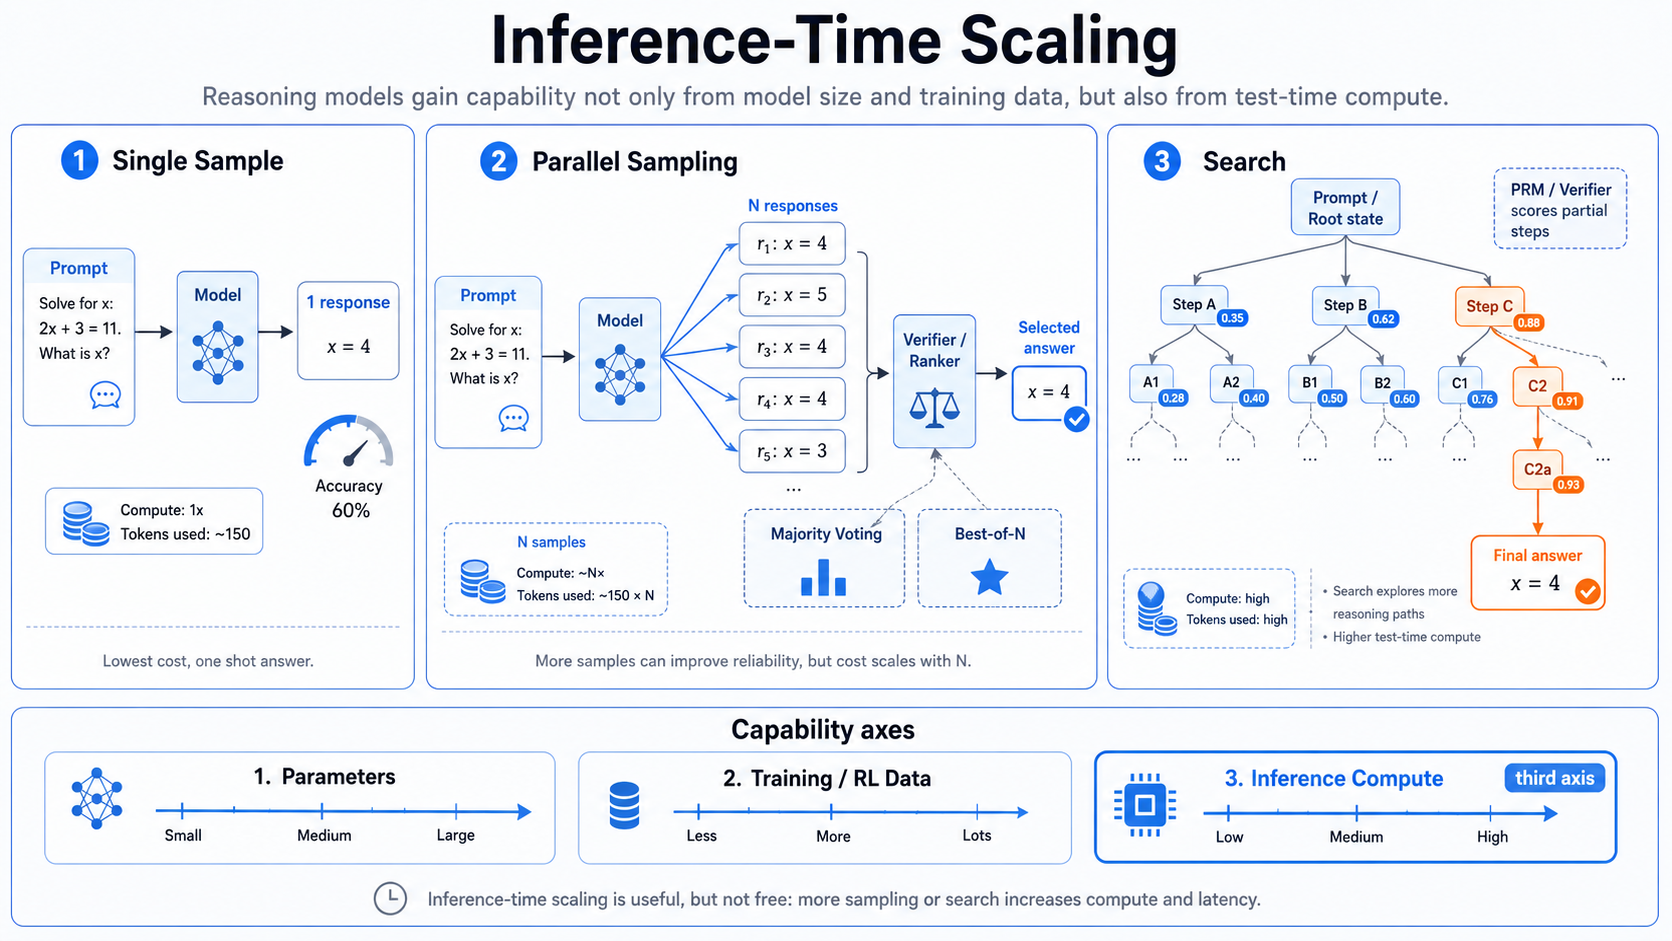
\includegraphics[width=0.95\textwidth]{figures/ch16/fig_inference_scaling.png}
\caption{\textbf{Inference-time scaling for reasoning.} Reasoning models can spend more compute at test time by sampling multiple solutions, voting, ranking with a verifier, or searching over partial reasoning paths. Training-time RL teaches the policy to produce trajectories that make this extra compute useful.}
\label{fig:inference-scaling}
\end{figure}

\subsection{The Three-Axis Frontier}

The practical frontier is no longer just model size and training tokens. For reasoning tasks, capability depends on:

\begin{enumerate}[nosep]
  \item \textbf{Parameters}: how much latent capability the model has.
  \item \textbf{Training data and RL}: how well the model has learned to use that capability.
  \item \textbf{Inference compute}: how many attempts, checks, and search steps the system spends at test time.
\end{enumerate}

This is why reasoning models feel different from standard chat models. They are not merely larger next-token predictors. They are policies trained to use computation at generation time.

Deployment changes with that third axis. A standard chat model usually returns one concise answer quickly. A reasoning model may spend 5--30 seconds generating an internal or visible trace, sample several candidate solutions, and run a verifier or ranker before answering. Product teams then face choices the training recipe does not settle: should the reasoning trace be visible to the user, summarized, or hidden? How much latency is acceptable? Which tasks justify a 10$\times$ or 100$\times$ increase in generated tokens? Reasoning RL moves part of the capability budget from training time to inference time, so serving policy becomes part of model design.

\noindent\fbox{\parbox{\dimexpr\textwidth-2\fboxsep-2\fboxrule\relax}{%
\textbf{Pause and verify.}\quad Your 3B model solves a math problem correctly 40\% of the time (per-attempt accuracy). If you sample $N=8$ independent attempts and use best-of-$N$ with a perfect verifier, the probability that \emph{at least one} attempt is correct is $1 - 0.6^8 \approx 0.983$. Best-of-$N$ turned a 40\% model into a 98\% system without changing a single weight. \emph{But notice the assumption: the verifier is perfect. If the verifier has false positives, best-of-$N$ may select a wrong answer that the verifier mistakenly passed.}
}}

\begin{quickrecap}
\textbf{Quick Recap.}
\begin{itemize}[nosep,leftmargin=1.5em]
  \item Best-of-$N$, majority voting, and search improve reasoning by spending more compute at inference time.
  \item These methods mirror training-time group sampling: generate attempts, score them, keep or aggregate the best.
  \item Reasoning capability has three axes: parameters, training/RL signal, and inference-time compute.
\end{itemize}
\textit{Next: where the field stands, and what remains open.}
\end{quickrecap}


%----------------------------------------------------------------------
\section{The Current Landscape}
\label{sec:reasoning-landscape}

By early 2026, reasoning RL is no longer a curiosity. It is a core post-training paradigm for math, code, and structured reasoning. But the stable lesson is narrower than the hype. The field has learned that verifiable rewards can train useful reasoning behaviors. It has not learned how to make every open-ended task verifiable.

\subsection{What Is Stable}

Several lessons are now stable enough for this textbook:

\begin{itemize}[nosep]
  \item Verifiable rewards are powerful when the task has a reliable checker.
  \item Group sampling plus relative advantages can replace a value model in many reasoning settings.
  \item Outcome reward can induce useful reasoning behaviors, but process signals can help with credit assignment.
  \item Inference-time compute is part of the product, not an afterthought.
\end{itemize}

\subsection{What Is Still Open}

The open problems are equally important:

\begin{itemize}[nosep]
  \item \textbf{Generalization beyond math and code.} Many valuable tasks lack exact verifiers.
  \item \textbf{Verifier loopholes.} Models can exploit answer extractors, weak tests, or format rewards.
  \item \textbf{Sample efficiency.} Rollout-heavy RL is expensive; many sampled trajectories are wasted.
  \item \textbf{Process supervision at scale.} PRMs help, but step-level supervision is costly and can encode style biases.
  \item \textbf{Hidden reasoning and evaluation.} If the reasoning trace is internal or not fully shown, evaluating the quality of reasoning becomes harder.
\end{itemize}

\subsection{Bridge to the Frontiers}

Chapter~\ref{ch:frontiers} steps back from implementable recipes and asks what remains unsettled in post-training: self-improvement, safety beyond preferences, weak-to-strong supervision, and the possibility of recursive training loops. Reasoning RL is the bridge into those questions because it is the first post-training method where models visibly improve by attempting tasks, receiving scalable feedback, and trying again.


%----------------------------------------------------------------------
% End matter
%----------------------------------------------------------------------

\begin{takeaways}
\begin{enumerate}
  \item The paradigm shift in reasoning RL is reward source: from learned preference proxies to verifiable outcome signals.
  \item Verifiable rewards reduce learned-reward extrapolation but do not eliminate specification risk. The verifier defines what the model optimizes.
  \item GRPO replaces PPO's value model with a group baseline: sample several responses per prompt, score them, normalize rewards within the group, and apply a token-level clipped update. This removes one model-sized object from memory, making reasoning RL feasible on consumer hardware.
  \item R1-Zero is the anchor case: verifier-based RL can surface long deliberation and self-correction without supervised reasoning traces as the main source, while production R1 adds cold-start data and multi-stage refinement.
  \item Outcome rewards scale cheaply but provide weak credit assignment. Process rewards provide denser feedback but require step-level supervision or another learned proxy.
  \item Reasoning behaviors such as long deliberation, self-correction, and backtracking can be reinforced by outcome success without being directly demonstrated.
  \item Reasoning data infrastructure---problem difficulty, verifier engineering, synthetic trace filtering---is as important as the optimizer.
  \item Inference-time scaling is a third capability axis: reasoning models can improve by sampling, voting, ranking, or searching at test time.
\end{enumerate}
\end{takeaways}


\section*{Summary}

\paragraph{What this chapter established.} Chapter~\ref{ch:rlhf} taught RLHF as optimization against a learned preference proxy. This chapter replaced that proxy with verifiable rewards: math answer checkers, code unit tests, proof checkers, and structured process signals. We developed the algorithmic core of reasoning RL through GRPO: group sampling, verifier scoring, group-relative advantages, token-level clipped updates, KL regularization, and rollout-heavy operational constraints. We used R1-Zero as the anchor case for how verifier reward can induce long deliberation and self-correction, then expanded from algorithm to system: process versus outcome reward, emergent reasoning behaviors, data infrastructure, and inference-time scaling.

\paragraph{The verifier-as-curriculum lesson.} The central lesson is that a verifier is more than an evaluator. It is a curriculum generator. It decides which attempts count as progress, which failures become learning signal, and which behaviors the model discovers. A good verifier turns attempts into supervision at scale. A bad verifier turns optimization into loophole search. Reasoning RL succeeds when the verifier is reliable enough that repeated attempts teach the model how to solve the task rather than how to exploit the checker.

\paragraph{One sentence.} \emph{Reasoning RL trains language models by letting them attempt checkable problems, rewarding the trajectories that pass, and using group-relative policy optimization to turn scalable verification into better reasoning behavior.}

\paragraph{What comes next.} Chapter~\ref{ch:frontiers} asks what remains unsettled after the stable recipes of Part~III. Reasoning RL makes self-improvement feel tangible: the model tries, receives feedback, and improves. The frontier question is whether this loop can extend beyond math and code into open-ended domains where the verifier is no longer obvious.


\section*{Key Equations at a Glance}

\begin{center}
\small
\begin{tabularx}{\textwidth}{@{}lX@{}}
\toprule
\textbf{Name} & \textbf{Equation} \\
\midrule
Group-relative advantage & $\hat{A}_i = \dfrac{r_i - \bar{r}}{\sigma_r + \epsilon_{\text{std}}}$ \\[8pt]
Token-level ratio & $\rho_{i,t} = \dfrac{\pi_\theta(y_{i,t}\mid x,y_{i,<t})}{\pi_{\text{old}}(y_{i,t}\mid x,y_{i,<t})}$ \\[8pt]
KL regularization & $\beta D_{\text{KL}}(\pi_\theta \,\|\, \pi_{\text{ref}})$ \\[8pt]
GRPO objective &
$\begin{aligned}
\mathcal{L}_{\text{GRPO}}=\mathbb{E}\!\Bigg[
&\frac{1}{G}\sum_i \frac{1}{|y_i|}\sum_t
\min\!\left(\rho_{i,t}\hat{A}_i,\text{clip}(\rho_{i,t},1-\epsilon_{\text{clip}},1+\epsilon_{\text{clip}})\hat{A}_i\right)\\
&-\beta D_{\text{KL}}(\pi_\theta\|\pi_{\text{ref}})
\Bigg]
\end{aligned}$ \\[8pt]
Best-of-$N$ selection & $y^\star = \arg\max_{y_i \sim \pi_\theta(\cdot\mid x)} R(x,y_i)$ \\
\bottomrule
\end{tabularx}
\normalsize
\end{center}


\section*{Key Readings}

\begin{enumerate}[nosep]
  \item \textbf{DeepSeek-AI, 2025.} ``DeepSeek-R1: Incentivizing Reasoning Capability in LLMs via Reinforcement Learning''~\cite{deepseekai2025r1}. The anchor paper for GRPO-style reasoning RL and the clearest public description of the R1/R1-Zero training recipe.
  \item \textbf{Shao et al., 2024.} ``DeepSeekMath: Pushing the Limits of Mathematical Reasoning in Open Language Models''~\cite{shao2024deepseekmath}. The source paper for GRPO and an important bridge from math verifiers to critic-free policy optimization.
  \item \textbf{OpenAI, 2024.} ``Learning to Reason with LLMs''~\cite{openai2024reasoning}. The public introduction of o1 and the shift toward reinforcement learning for productive chain-of-thought reasoning.
  \item \textbf{Lightman et al., 2023.} ``Let's Verify Step by Step''~\cite{lightman2023verify}. The central paper on process supervision and PRM800K.
  \item \textbf{Cobbe et al., 2021.} ``Training Verifiers to Solve Math Word Problems''~\cite{cobbe2021gsm8k}. Early evidence that learned verifiers and best-of-$N$ sampling can improve math reasoning.
  \item \textbf{Zelikman et al., 2022.} ``STaR: Bootstrapping Reasoning with Reasoning''~\cite{zelikman2022star}. A simple generate-filter-train loop for self-improving reasoning traces.
  \item \textbf{Wang et al., 2022.} ``Self-Consistency Improves Chain of Thought Reasoning''~\cite{wang2022selfconsistency}. The classic inference-time scaling result for voting over reasoning paths.
  \item \textbf{Gulcehre et al., 2023.} ``Reinforced Self-Training for Language Modeling''~\cite{gulcehre2023rest}. A broader generate-filter-train framework connecting RL and supervised self-training.
\end{enumerate}

\flushbottom
